% MAGNET -- arXiv draft, third version. Compile: ~/miniconda3/envs/tex/bin/tectonic -X compile main.tex (from paper/).
% Figures: python paper/make_fig_layouts.py mnist|fmnist ; python paper/make_fig_ablations.py ; python paper/make_fig_tail.py
% Tables: python paper/make_tables.py (from benchmarks/BENCHMARK.md), benchmarks/seeds_summary.py, benchmarks/global_strata.py,
% benchmarks/graph_table.py --table-only, benchmarks/staged_seeds.py.
\documentclass[11pt]{article}
\usepackage[margin=1in]{geometry}
\usepackage{amsmath,amssymb,booktabs,graphicx,xcolor,hyperref,natbib,enumitem,microtype}
\usepackage[font=small]{caption}
\graphicspath{{figures/}}
\newcommand{\todo}[1]{\textcolor{red}{[#1]}}
\newcommand{\magnet}{\textsc{magnet}}
\setlist{nosep}

\title{\magnet: staged neighbour embedding\\ with scale-matched refinement}
\author{Maixent Chenebaux\thanks{\texttt{github.com/kerighan/lib-magnet}, package \texttt{magnet-learn}.}}
\date{Draft, \today}

\begin{document}
\maketitle

\begin{abstract}
We study a staged neighbour-embedding procedure: a layout is first built by sampled optimisation
(UMAP's objective with negative sampling) under a transient mid-range attraction, then refined by a
scale-matched $t$-SNE objective computed in full batch with an FFT-interpolated repulsion. On MNIST and
Fashion-MNIST 70k, a 300-iteration refinement started at the full-batch optimiser's own scale and
without early exaggeration raises the 15-NN preservation of the start to the full-batch level
(0.353--0.356 and 0.327--0.330) while retaining most of its pairwise-distance Spearman correlation
(within $-0.02$ / $+0.03$). The same refinement does the same to UMAP and PaCMAP starts, and openTSNE's
optimiser can carry it out on our start. The first stage's distance Spearman is set by the mid-range
attraction, not by the sampled estimator: without it the sampled layout scores below openTSNE. With a
stiff attraction, \magnet{}'s start has the highest pairwise Spearman among the default
neighbour-embedding starts we tested, but not the best class-centroid geometry, and the stiffness
makes that geometry variable. The hybrid reaches 0.353 / 0.455 and 0.328 / 0.750 in 15-NN preservation
/ Spearman over five runs, at 1.3 times UMAP's runtime and a ninth of openTSNE's on the same machine.
The implementation (C++ NN-descent, lock-free SGD, split attraction and repulsion exponents, FFT
repulsion) is the fastest CPU method on the twelve-method panel on the four tabulated data sets; the
result is not universal (the hybrid trails Barnes--Hut $t$-SNE on 20 newsgroups), and PCA remains
stronger than every neighbour embedding on pairwise-distance correlation on the real data sets.
\end{abstract}

\section{Introduction}
A neighbour embedding attracts the ends of the edges of a kNN graph and repels everything else, and the
balance of the two forces is the one axis that separates $t$-SNE, UMAP and LargeVis
\citep{boehm2022attraction, damrich2021umap}. Layouts that keep neighbourhoods tight (the $t$-SNE
family) and layouts that keep the arrangement of the clusters (sampled optimisers with an informative
start or a mid-range term) are usually obtained from different programs, and the knobs that move one
program towards the other (exaggeration, a heavier tail, a spring) buy one side with the other. This
paper studies the alternative of running two stages in sequence and asks what each stage contributes.

The contributions, with their scope stated:
\begin{enumerate}[leftmargin=2em]
\item \textbf{A staged procedure and its hand-over} (Sec.~\ref{sec:staged}). A sampled first stage
  under a mid-range attraction, then a short full-batch $t$-SNE refinement started at that optimiser's
  own scale, without early exaggeration and without the attraction. This differs from the informative
  initialisation of \citet{kobak2021init} in the hand-over scale (the start is kept at the full-batch
  layout's scale rather than shrunk to $t$-SNE's tiny initialisation) and in dropping exaggeration. We
  report the configurations that were tested and which of them fail; we do not claim that the tested
  conditions are necessary.
\item \textbf{Controls that say where the gain comes from} (Sec.~\ref{sec:stagedbase}). Applied to
  UMAP, PaCMAP, openTSNE and our own starts, the refinement brings every one of them to the full-batch
  15-NN level and leaves their pairwise Spearman ordering intact; the global column after the pass is
  predominantly the global column of the start. An ablation shows that the first stage's global
  structure is the mid-range attraction's, not the sampled estimator's. A $2 \times 2$ design
  (\magnet{} and PaCMAP starts, weak and stiff mid-range attraction, five runs each) tests whether the
  start matters beyond that attraction.
\item \textbf{A fast implementation with audited protocols} (Sec.~\ref{sec:exp}): MNIST 70k in 3.6~s for
  the sampled mode, 8~s for the full-batch mode, 11~s for the sequence, against 8~s for UMAP and 94~s
  for openTSNE on an idle 20-thread machine. The baselines' timings are audited (numba warm-up, UMAP's
  single-threaded seeded path, PaCMAP's seeded path, a per-phase breakdown of openTSNE, the protocol for
  graph inputs). The speed claim is restricted to the panel; uwot is not in it.
\item \textbf{What the global metric measures} (Sec.~\ref{sec:global}): split by class and by distance
  tercile and reduced to the class centroids, the pairwise Spearman and the centroid Spearman rank the
  methods differently, PCA leads every neighbour embedding on both, and the hybrid is last of the
  neighbour embeddings on the centroids of MNIST.
\end{enumerate}
A secondary contribution is the split of the kernel exponent into an attraction exponent and a
repulsion exponent, which the implementation uses and which removes a \texttt{pow} from the inner loop
at the default exponents; the asymptotic arguments for it and the measured optima are summarised in
Sec.~\ref{sec:theory} and given in full in Appendix~\ref{app:theory}. Figure~\ref{fig:layouts} shows
the six layouts of MNIST 70k that the paper returns to.

\begin{figure}[t]
\centering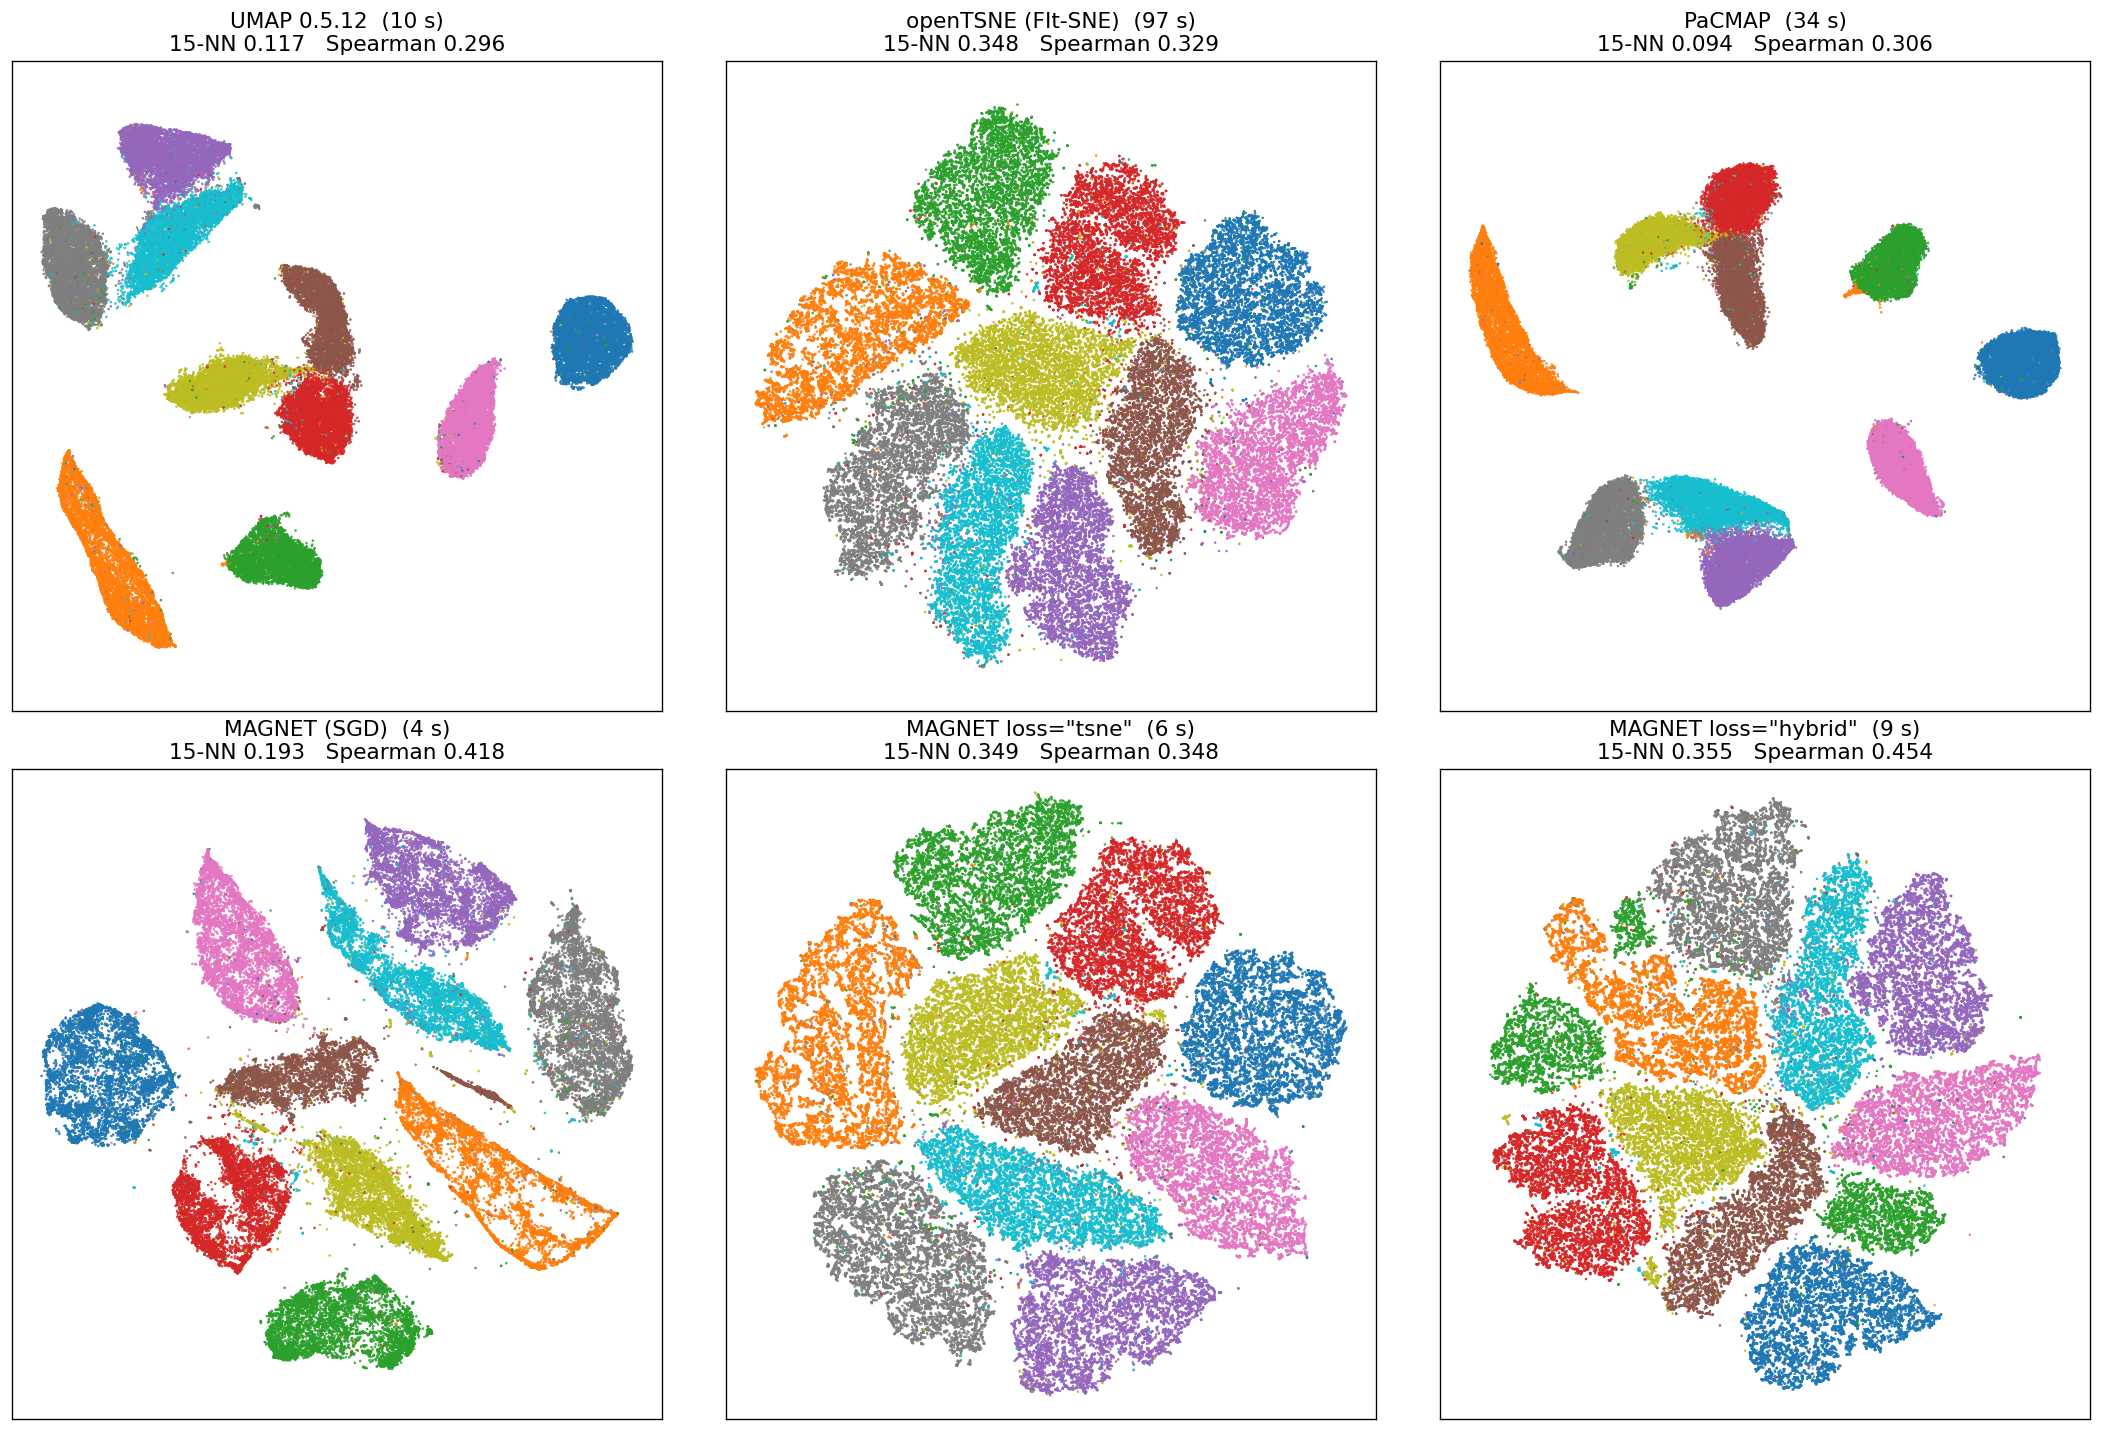
\includegraphics[width=\textwidth]{layouts_mnist.png}
\caption{MNIST 70k under six methods, same seed. Top: UMAP, openTSNE (FIt-SNE), PaCMAP. Bottom:
\magnet{} sampled (SGD), full-batch (FFT repulsion), hybrid (SGD layout refined by the full-batch pass).
Time, 15-NN preservation and distance Spearman in the panel titles (single runs, 20 threads on a shared
machine, numba compilation excluded). Fashion-MNIST: Fig.~\ref{fig:layouts_fmnist}.}
\label{fig:layouts}
\end{figure}

\section{Objectives and algorithm}\label{sec:algo}
\paragraph{Graph.} The input is UMAP's fuzzy-union kNN graph ($k = 15$) with weights $w_{ij} \in (0, 1]$,
symmetric, built by a C++ NN-descent (1.2~s for $70\mathrm{k} \times 784$) or by a scatter/gather
NN-descent for sparse rows (Appendix~\ref{app:impl}).

\paragraph{Sampled objective (first stage).} UMAP's cross-entropy with negative sampling: for an edge
$(i, j)$ sampled with probability proportional to $w_{ij}$ the attraction $-\log \phi_b(d_{ij})$ is
applied, with $\phi_b(d) = 1/(1 + a d^{2b})$, followed by five negatives $l$ drawn uniformly with the
repulsion $-\gamma \log (1 - \phi_{b_r}(d_{il}))$, $\gamma = 2$; the two kernels carry separate
exponents $b = 0.6$ and $b_r = 1$ (Sec.~\ref{sec:theory}), $a$ is UMAP's for the given spread and
\texttt{min\_dist}. Both ends of an edge move; the gradient is clipped at 4 as in UMAP; updates are
lock-free across threads; the epoch schedule is UMAP's. \emph{Mid-range attraction:} with probability
$1/4$ a positive sample is followed by a partner $m$ of $i$ drawn from five PaCMAP-style mid-near pairs
(the second closest of six random rows in the data space, \citealp{wang2021pacmap}; on graphs, the end
of a short random walk), and $i$ is pulled towards $m$ with a linear spring of stiffness $s$, annealed
linearly to zero over the first half of the epochs. $s = 0.1$ by default, $0.5$ in the hybrid. The
initialisation is spectral (Chebyshev-filtered subspace iteration).

\paragraph{Full-batch objective (second stage, and \texttt{loss="tsne"}).} The Kullback--Leibler
divergence $\sum_{ij} p_{ij} \log (p_{ij} / q_{ij})$ with $p_{ij} = w_{ij} / \sum w$ on the same graph
and $q_{ij} = (1 + d_{ij}^2)^{-1} / Z$, $Z = \sum_{k \ne l} (1 + d_{kl}^2)^{-1}$: $t$-SNE's objective on
the fuzzy graph instead of perplexity-calibrated affinities. The gradient is computed in full batch,
the repulsive sum by the FFT interpolation of \citet{linderman2019fitsne} (three interpolation points per
box of width 1 in layout units; accuracy checked against the exact sum in Appendix~\ref{app:impl}),
with $t$-SNE's momentum and gains and learning rate $n / 12$. Used alone (\texttt{loss="tsne"}) it runs
600 iterations with early exaggeration 12 for the first 200 from a PCA initialisation of standard
deviation $10^{-4}$.

\paragraph{The sequence (\texttt{loss="hybrid"}).} The first stage with $s = 0.5$; the layout is
centred and rescaled to standard deviation $\sigma = 31 \sqrt{n / 70000}$ (the scale the full-batch
mode reaches on its own at 70k points); then 300 iterations of the second stage with exaggeration 1
throughout, momentum 0.8, no mid-range attraction. The hand-over scale is a rescaling of the start, not
a re-initialisation.

The kernel scale of the sampled objective is $d_k = a^{-1/2b}$: 0.78 at UMAP's defaults
($a = 1.58$, $b = 0.9$), 0.66 at \magnet{}'s ($a = 1.64$, $b = 0.6$). Graphs and sparse matrices are
accepted directly; \texttt{transform()} places new points. Engineering details (the lock-free and the
owner-parallel SGD kernels, the sparse search, the cost at 1M points) are in Appendix~\ref{app:impl}.

\section{Staged refinement}\label{sec:staged}
\subsection{Hand-over: what was tested}\label{sec:handover}
The sampled mode has the highest pairwise Spearman among the neighbour embeddings of the benchmark and
the full-batch mode the highest 15-NN preservation, and each is mediocre on the other axis (MNIST: 0.19
/ 0.41 against 0.35 / 0.35). Refining the sampled layout with the full-batch objective was tried under
the following settings, each on MNIST 70k from the same start:
\begin{itemize}[leftmargin=1.5em]
\item \emph{Scale.} From $t$-SNE's tiny initialisation (the start shrunk to $\sigma = 10^{-4}$, with
  exaggeration) the layout re-expands and loses the arrangement: Spearman 0.29--0.39. From the start's
  own scale ($\sigma \approx 4$) the normalised repulsion collapses it. From $\sigma = 15 / 31 / 62 /
  124$ with 300 iterations: 15-NN 0.338 / 0.353 / 0.357 / 0.338, Spearman 0.395 / 0.413 / 0.424 / 0.427
  for a start at 0.428, in 6 / 10 / 30 / 121~s (the FFT grid follows the layout's extent, so the cost of
  an iteration grows with the square of the scale). The default is 31; 62 keeps more of the start's
  Spearman at three times the cost, and 62 with 150 iterations keeps all of it (0.428) at 15-NN 0.349 in
  17~s. The rule $31 \sqrt{n / 70000}$ was set on 70k points and has not been validated at other sizes.
\item \emph{Exaggeration.} With early exaggeration 12 for the first 100 of 300 iterations the
  arrangement of the start is overwritten (Spearman 0.29--0.39 above, which combined the tiny scale and
  the exaggeration; the two were not separated, and we report them together).
\item \emph{Mid-range attraction in the second stage.} At stiffness 0.1 (not annealed) 15-NN falls to
  0.118 and Spearman to 0.310; at 0.5 the layout collapses ($\sigma = 2$, 15-NN 0.04). At the full-batch
  scale a linear spring is a strong contraction.
\item \emph{Iterations.} 25 / 75 / 150 / 300 / 600: 15-NN 0.277 / 0.328 / 0.343 / 0.353 / 0.352,
  Spearman 0.428 / 0.427 / 0.423 / 0.413 / 0.412. Section~\ref{sec:persist} follows the trace to 3000.
\item \emph{Learning rate} 1000 or 20000 instead of $n / 12$, and kernel degrees of freedom 0.5: no
  gain (15-NN 0.340 / 0.335 / 0.279).
\item \emph{Order.} Full-batch layout then 60--150 sampled epochs: Spearman 0.436 but 15-NN back at the
  sampled level (0.13--0.17).
\item \emph{One loss.} Inside the full-batch objective, a mid-range spring (linear or PaCMAP's bounded
  form), a constant-strength far-field repulsion added to the normalised one, and late exaggeration were
  each tried; each costs 15-NN before the Spearman moves (to 0.13 / 0.08 / 0.01 for springs of 0.3 / 1 /
  3; a window of a factor ten between no effect and a destroyed layout for the far-field term; 0.278 /
  0.195 / 0.121 for exaggeration 1.5 / 2 / 4, which buys compactness, not Spearman). These are finite
  negative results on one data set.
\end{itemize}
The configuration kept (scale 31, no exaggeration, no attraction, 300 iterations) gives 15-NN
0.353--0.356 and Spearman 0.411--0.416 from the default start ($s = 0.1$) and 0.353 $\pm$ 0.001 /
0.455 $\pm$ 0.014 from the stiff start ($s = 0.5$) over five runs (Table~\ref{tab:seeds}).

\paragraph{The first stage can be tuned for global structure alone.} Since the second stage rebuilds
the neighbourhoods, the local cost of a stiffer attraction in the first stage is erased and most of its
Spearman gain kept (Fig.~\ref{fig:hybrid}b): at $s = 0.5$ the start alone scores 0.178 / 0.459, the
sequence 0.356 / 0.442; at $s = 0.1$, 0.193 / 0.418 and 0.356 / 0.414 (single runs; the gap between the
two stiffnesses is 0.041 before the pass and 0.028 after). $s = 1.0$ reaches 0.478 before the pass on
MNIST but loses 0.04 of Spearman on the blobs; $s = 0.5$ is at or above $s = 0.1$ on 15-NN, Spearman and
triplets on the four data sets, and below it on the centroid Spearman of MNIST (Sec.~\ref{sec:global}).
A shorter first stage does not work (100 epochs: 0.276 after the pass).

\subsection{Staged baselines}\label{sec:stagedbase}
Is the gain the staging or the start? Table~\ref{tab:staged} applies the same pass to seven starts on
MNIST and Fashion-MNIST, the UMAP, PaCMAP and openTSNE starts being the seed-0 layouts of
Fig.~\ref{fig:layouts} (single runs; Table~\ref{tab:staged_seeds} repeats the decisive rows with five
runs). (i) Every neighbour-embedding start lands at 0.353--0.356 of 15-NN on MNIST and 0.327--0.330 on
Fashion-MNIST, the full-batch mode's own level, in 8--13~s. (ii) The pairwise Spearman moves by
$-0.021$ to $+0.035$ (it rises for UMAP and PaCMAP on Fashion-MNIST, falls most for our stiff start), so
the ordering of the starts on that column survives the pass and the column after the pass is
predominantly the column of the start; the centroid Spearman moves by $-0.07$ to $+0.01$, and the two
starts with the best centroids (UMAP, PaCMAP) lose the most. (iii) A start without neighbourhoods is
not fully repaired by 300 iterations: PCA-2 reaches 0.315 (from 0.010) and loses 0.07--0.09 of
Spearman; a random start reaches 0.065. (iv) Handed our stiff start at the same scale, openTSNE's
optimiser with its own perplexity-30 affinities (300 iterations, momentum 0.8, no exaggeration) reaches
0.346 / 0.428 on MNIST and 0.322 / 0.743 on Fashion-MNIST, 4.7 and 5.7 times slower at 4 threads; on
the PCA start it does better than our pass on 15-NN (0.333 against 0.315). The two backends are not
interchangeable (affinities and optimiser both differ), but the hand-over transfers.

\begin{table}[t]
\centering\small
\caption{Staged baselines (\texttt{staged\_baselines.py}, 4 threads, single runs). The same full-batch
pass (300 iterations, no exaggeration, no spring, hand-over scale 31) applied to seven starts; 15-NN
preservation, distance Spearman and centroid Spearman before $\to$ after, and the time of the pass. Last
rows: the same starts handed to openTSNE's optimiser for 300 iterations.}
\label{tab:staged}
\footnotesize
\begin{tabular}{llrrrr}
\toprule
data & start & 15-NN & Spearman & centroids & pass (s) \\
\midrule
MNIST & PCA-2 & 0.010 $\to$ 0.315 & 0.488 $\to$ 0.399 & 0.814 $\to$ 0.811 & 15.9 \\
 & random & 0.000 $\to$ 0.065 & 0.000 $\to$ 0.008 & 0.31 $\to$ 0.33 & 29.0 \\
 & UMAP & 0.117 $\to$ 0.353 & 0.296 $\to$ 0.299 & 0.752 $\to$ 0.681 & 9.9 \\
 & PaCMAP & 0.094 $\to$ 0.354 & 0.306 $\to$ 0.311 & 0.684 $\to$ 0.633 & 11.4 \\
 & openTSNE & 0.348 $\to$ 0.354 & 0.329 $\to$ 0.326 & 0.607 $\to$ 0.614 & 11.8 \\
 & \magnet{} SGD, $s = 0.1$ & 0.193 $\to$ 0.356 & 0.418 $\to$ 0.414 & 0.635 $\to$ 0.617 & 13.1 \\
 & \magnet{} SGD, $s = 0.5$ (hybrid) & 0.178 $\to$ \textbf{0.356} & 0.459 $\to$ \textbf{0.442} & 0.524 $\to$ 0.492 & 11.8 \\
 & \magnet{} SGD, $s = 0.5$ $\to$ openTSNE & 0.178 $\to$ 0.346 & 0.459 $\to$ 0.428 & 0.524 $\to$ 0.507 & 55.2 \\
 & PCA-2 $\to$ openTSNE & 0.010 $\to$ 0.333 & 0.488 $\to$ 0.376 & 0.814 $\to$ 0.756 & 60.2 \\
\midrule
Fashion & PCA-2 & 0.018 $\to$ 0.315 & 0.873 $\to$ 0.799 & 0.971 $\to$ 0.962 & 9.1 \\
 & random & 0.000 $\to$ 0.062 & 0.007 $\to$ 0.028 & 0.11 $\to$ 0.21 & 28.2 \\
 & UMAP & 0.133 $\to$ \textbf{0.330} & 0.572 $\to$ 0.607 & 0.879 $\to$ 0.879 & 8.2 \\
 & PaCMAP & 0.098 $\to$ 0.327 & 0.582 $\to$ 0.599 & 0.885 $\to$ 0.882 & 7.5 \\
 & openTSNE & 0.323 $\to$ 0.329 & 0.617 $\to$ 0.614 & 0.882 $\to$ 0.876 & 8.7 \\
 & \magnet{} SGD, $s = 0.1$ & 0.203 $\to$ 0.328 & 0.729 $\to$ 0.716 & 0.939 $\to$ 0.908 & 8.3 \\
 & \magnet{} SGD, $s = 0.5$ (hybrid) & 0.193 $\to$ 0.329 & 0.774 $\to$ \textbf{0.753} & 0.958 $\to$ 0.931 & 7.7 \\
 & \magnet{} SGD, $s = 0.5$ $\to$ openTSNE & 0.193 $\to$ 0.322 & 0.774 $\to$ 0.743 & 0.958 $\to$ 0.924 & 44.1 \\
 & PCA-2 $\to$ openTSNE & 0.018 $\to$ 0.316 & 0.873 $\to$ 0.770 & 0.971 $\to$ 0.956 & 40.9 \\
\bottomrule
\end{tabular}
\end{table}

\paragraph{Where the first stage's global structure comes from.} Without the mid-range attraction the
sampled layout of MNIST scores Spearman 0.285, below openTSNE (0.330) and below the full-batch mode
(0.348); at $s = 0.1 / 0.3 / 1.0$ it scores 0.413 / 0.427 / 0.478 at 15-NN 0.193 / 0.187 / 0.168
(Fig.~\ref{fig:hybrid}a). The sampled estimator by itself does not give the first stage its lead on
that column; the attraction does. openTSNE is above UMAP on pairwise Spearman on all four data sets
(0.330 / 0.617 / 0.106 / 0.382 against 0.297 / 0.571 / 0.099 / 0.079), so ``sampled optimisers keep the
arrangement'' is not what the tables say either; what they say is that a transient mid-range attraction
in a sampled optimiser raises the pairwise Spearman, and that the refinement keeps most of it.

\subsection{Is the start \magnet{}'s, or the attraction's?}\label{sec:twobytwo}
The comparison of starts in Table~\ref{tab:staged} sets our first stage at a stiffness chosen on these
data against UMAP and PaCMAP at their defaults, and PaCMAP has a mid-near term of its own.
Table~\ref{tab:staged_seeds} runs a $2 \times 2$ design with five runs per cell: \magnet{}'s first stage
at $s = 0$, 0.1, 0.5 and 1.0, PaCMAP at its defaults and at a stiff mid-near setting chosen by a sweep of
its \texttt{MN\_ratio} and phase lengths on MNIST and frozen before Fashion-MNIST
(\texttt{pacmap\_sweep.py}), plus UMAP and openTSNE, every start going through the same pass.
The sweep's best PaCMAP setting (\texttt{MN\_ratio} 4, the default phase lengths) raises its
Spearman before the pass from 0.310 to 0.319 on MNIST and from 0.582 to 0.624 on Fashion-MNIST; the
other settings of the sweep are between 0.24 and 0.33. After the same pass, the stiff PaCMAP start
reaches 0.346 $\pm$ 0.017 on MNIST and 0.648 $\pm$ 0.001 on Fashion-MNIST, against 0.449 $\pm$ 0.015
and 0.750 $\pm$ 0.001 for our first stage at $s = 0.5$ (0.456 / 0.764 at $s = 1.0$), 0.310 / 0.605 for
UMAP and 0.327 / 0.617 for openTSNE. Our first stage without the attraction ($s = 0$) lands at 0.301 /
0.588, below UMAP on MNIST. So the start matters beyond the attraction's presence: PaCMAP's mid-near
term, stiffened with the same tuning budget, does not reach the same pairwise Spearman, and the
difference (0.10 on both data sets) is many standard deviations wide. What the start pays is visible in
the last column: on MNIST the centroid Spearman after the pass is 0.466 $\pm$ 0.158 at $s = 0.5$ and
0.499 $\pm$ 0.080 at $s = 1.0$, against 0.628 $\pm$ 0.016 at $s = 0.1$, 0.664 $\pm$ 0.013 for UMAP and
0.687 $\pm$ 0.020 for stiff PaCMAP; on Fashion-MNIST the stiff start is best on that column too
(0.934 / 0.943). The pass itself adds 0.01--0.03 of Spearman to UMAP and PaCMAP starts and takes
0.01--0.02 from ours, on both data sets, in every run.

\begin{table}[t]
\centering\small
\caption{The $2 \times 2$ design with seeds (\texttt{staged\_seeds.py}, all cores, 5 runs per cell; 2
for openTSNE): the same pass applied to \magnet{}'s first stage at four stiffnesses, PaCMAP at its
defaults and at the stiff setting of the sweep, UMAP and openTSNE. Before $\to$ after (mean), $\pm$
standard deviation of the value after the pass.}
\label{tab:staged_seeds}
\resizebox{\textwidth}{!}{\begin{tabular}{llrrrrr}
\toprule
data & start & $n$ & 15-NN & Spearman & triplets & centroids \\
\midrule
MNIST & \magnet{} SGD, spring 0 & 5 & 0.205 $\to$ 0.355 $\pm$ 0.001 & 0.276 $\to$ 0.301 $\pm$ 0.004 & 0.604 $\to$ 0.610 $\pm$ 0.001 & 0.723 $\to$ 0.659 $\pm$ 0.012 \\
MNIST & \magnet{} SGD, spring 0.1 & 5 & 0.193 $\to$ 0.355 $\pm$ 0.001 & 0.415 $\to$ 0.412 $\pm$ 0.004 & 0.645 $\to$ 0.643 $\pm$ 0.001 & 0.639 $\to$ 0.628 $\pm$ 0.016 \\
MNIST & \magnet{} SGD, spring 0.5 & 5 & 0.179 $\to$ 0.354 $\pm$ 0.002 & 0.463 $\to$ 0.449 $\pm$ 0.015 & 0.658 $\to$ 0.654 $\pm$ 0.005 & 0.479 $\to$ 0.466 $\pm$ 0.158 \\
MNIST & \magnet{} SGD, spring 1.0 & 5 & 0.169 $\to$ 0.352 $\pm$ 0.002 & 0.473 $\to$ 0.456 $\pm$ 0.027 & 0.662 $\to$ 0.657 $\pm$ 0.008 & 0.504 $\to$ 0.499 $\pm$ 0.080 \\
MNIST & PaCMAP default & 5 & 0.094 $\to$ 0.354 $\pm$ 0.001 & 0.310 $\to$ 0.321 $\pm$ 0.013 & 0.614 $\to$ 0.616 $\pm$ 0.004 & 0.682 $\to$ 0.643 $\pm$ 0.033 \\
MNIST & PaCMAP stiff (MN 4.0, iters (100, 100, 250)) & 5 & 0.093 $\to$ 0.353 $\pm$ 0.000 & 0.319 $\to$ 0.346 $\pm$ 0.017 & 0.619 $\to$ 0.624 $\pm$ 0.004 & 0.729 $\to$ 0.687 $\pm$ 0.020 \\
MNIST & UMAP default & 5 & 0.117 $\to$ 0.353 $\pm$ 0.001 & 0.301 $\to$ 0.310 $\pm$ 0.007 & 0.608 $\to$ 0.611 $\pm$ 0.002 & 0.745 $\to$ 0.664 $\pm$ 0.013 \\
MNIST & openTSNE default & 2 & 0.347 $\to$ 0.355 $\pm$ 0.001 & 0.330 $\to$ 0.327 $\pm$ 0.002 & 0.619 $\to$ 0.618 $\pm$ 0.000 & 0.606 $\to$ 0.611 $\pm$ 0.005 \\
\midrule
Fashion & \magnet{} SGD, spring 0 & 5 & 0.211 $\to$ 0.329 $\pm$ 0.001 & 0.566 $\to$ 0.588 $\pm$ 0.013 & 0.731 $\to$ 0.735 $\pm$ 0.005 & 0.871 $\to$ 0.868 $\pm$ 0.016 \\
Fashion & \magnet{} SGD, spring 0.1 & 5 & 0.204 $\to$ 0.327 $\pm$ 0.001 & 0.725 $\to$ 0.709 $\pm$ 0.004 & 0.784 $\to$ 0.776 $\pm$ 0.001 & 0.936 $\to$ 0.903 $\pm$ 0.005 \\
Fashion & \magnet{} SGD, spring 0.5 & 5 & 0.192 $\to$ 0.328 $\pm$ 0.000 & 0.773 $\to$ 0.750 $\pm$ 0.001 & 0.810 $\to$ 0.797 $\pm$ 0.001 & 0.958 $\to$ 0.934 $\pm$ 0.002 \\
Fashion & \magnet{} SGD, spring 1.0 & 5 & 0.183 $\to$ 0.330 $\pm$ 0.001 & 0.789 $\to$ 0.764 $\pm$ 0.003 & 0.818 $\to$ 0.805 $\pm$ 0.001 & 0.964 $\to$ 0.943 $\pm$ 0.002 \\
Fashion & PaCMAP default & 5 & 0.099 $\to$ 0.327 $\pm$ 0.001 & 0.582 $\to$ 0.600 $\pm$ 0.002 & 0.729 $\to$ 0.728 $\pm$ 0.001 & 0.883 $\to$ 0.884 $\pm$ 0.001 \\
Fashion & PaCMAP stiff (MN 4.0, iters (100, 100, 250)) & 5 & 0.097 $\to$ 0.329 $\pm$ 0.000 & 0.624 $\to$ 0.648 $\pm$ 0.001 & 0.746 $\to$ 0.748 $\pm$ 0.000 & 0.904 $\to$ 0.891 $\pm$ 0.003 \\
Fashion & UMAP default & 5 & 0.134 $\to$ 0.331 $\pm$ 0.001 & 0.572 $\to$ 0.605 $\pm$ 0.004 & 0.728 $\to$ 0.734 $\pm$ 0.001 & 0.879 $\to$ 0.882 $\pm$ 0.002 \\
Fashion & openTSNE default & 2 & 0.323 $\to$ 0.330 $\pm$ 0.000 & 0.619 $\to$ 0.617 $\pm$ 0.001 & 0.733 $\to$ 0.732 $\pm$ 0.000 & 0.882 $\to$ 0.875 $\pm$ 0.000 \\
\bottomrule
\end{tabular}
}
\end{table}

\subsection{Persistence}\label{sec:persist}
Three hundred iterations keeping the start's Spearman does not show that the full-batch objective
preserves it at convergence. Table~\ref{tab:persist} follows the pass from the stiff start to 3000
iterations and from PCA-2 to 1200 (\texttt{k15\_persistence.py}, all cores). From the stiff start the
Spearman drifts from 0.480 to 0.470 at 300, 0.462 at 600, 0.455 at 1200 and 0.446 at 3000 iterations,
while 15-NN rises from 0.346 to 0.367 and the layout expands (standard deviation 31 to 55); the
centroids stay at 0.49--0.51; the objective is still decreasing at 3000. The drift is slow (0.034 over a
tenfold longer pass) and leaves the layout far above every other start, but it is a drift: the
full-batch objective does not preserve the start's pairwise Spearman at convergence, the 300-iteration
pass stops before most of the loss. From PCA-2 the loss is faster (0.488 to 0.418 at 300, 0.377 at 1200)
and 15-NN reaches 0.344 at 1200: a start without neighbourhoods is repaired more slowly and pays more.
Section~\ref{sec:virial} gives the reason for the expansion and Sec.~\ref{sec:projected} a refinement
that cannot drift.

\begin{table}[t]
\centering\small
\caption{Persistence of the start's structure along the full-batch pass (MNIST 70k, all cores;
\texttt{k15\_persistence.py}). KL is the objective on the graph edges; $\sigma$ the layout's standard
deviation.}
\label{tab:persist}
\begin{tabular}{lrrrrrrr}
\toprule
start & iterations & time (s) & 15-NN & Spearman & triplets & centroids & $\sigma$ \\
\midrule
\magnet{} SGD, $s = 0.5$ & 0 & & 0.180 & 0.480 & 0.666 & 0.513 & 31.0 \\
 & 300 & 7 & 0.346 & 0.470 & 0.663 & 0.512 & 34.1 \\
 & 600 & 16 & 0.354 & 0.462 & 0.660 & 0.501 & 37.4 \\
 & 1200 & 39 & 0.361 & 0.455 & 0.658 & 0.486 & 42.9 \\
 & 3000 & 129 & 0.367 & 0.446 & 0.656 & 0.490 & 54.7 \\
\midrule
PCA-2 & 0 & & 0.010 & 0.488 & 0.668 & 0.814 & 31.0 \\
 & 300 & 11 & 0.312 & 0.418 & 0.652 & 0.811 & 32.2 \\
 & 600 & 19 & 0.332 & 0.388 & 0.646 & 0.790 & 34.4 \\
 & 1200 & 40 & 0.344 & 0.377 & 0.642 & 0.752 & 39.0 \\
\bottomrule
\end{tabular}
\end{table}

\subsection{Scale: a virial identity for the full-batch objective}\label{sec:virial}
Write $k_{ij} = (1 + s^2 d_{ij}^2)^{-1}$ for the kernel of the layout dilated by $s$, $Z = \sum_{i \ne j} k_{ij}$
and $u_{ij} = s^2 d_{ij}^2 / (1 + s^2 d_{ij}^2)$. Differentiating the objective $F(sY) = \sum p_{ij} \log p_{ij}
- \sum p_{ij} \log k_{ij} + \log Z$ in $\log s$ gives
\[
\frac{\partial F(sY)}{\partial \log s} = 2\Big(\mathbb{E}_p[u] - \mathbb{E}_q[u]\Big)
= 2\Big(\textstyle\sum_{ij} p_{ij} u_{ij} - 1 + \sum_{ij} k_{ij}^2 / Z\Big),
\]
so at any stationary point of the objective the $p$-weighted mean of $d^2/(1+d^2)$ over the edges equals its
$q$-weighted mean over all pairs. Both sides cost one FFT evaluation: $\sum k_{ij}^2$ is the potential of
the second FIt-SNE kernel with unit charges. The KL-optimal dilation $s^\ast$ of a start $Y_0$ is the root of
this identity along the ray $sY_0$; it depends on $P$ and on the shape of $Y_0$, and the ray may have no
root in a bracketed range.

Table~\ref{tab:virial} gives $s^\ast$ (in units of the start's standard deviation) for the starts of
Table~\ref{tab:staged} on MNIST 70k (\texttt{k17}, \texttt{k18}): 85--93 for our sampled starts, 10 for
PCA-2, about 120 for UMAP; the full-batch mode's own layout after its 600 iterations is itself far from
its equilibrium scale (the derivative is still $-0.05$ at 124, four times its standard deviation), which
is the slow expansion of Table~\ref{tab:persist}. On MNIST subsamples $s^\ast$ grows as $n^{0.42}$ (28 / 54 /
85 at 5k / 20k / 70k; Fashion-MNIST 53 / 81 at 20k / 70k), which is the form of the rule
$31\sqrt{n/70000}$ with a measured exponent in place of the assumed $1/2$. The identity explains three
observations: the pass expands every start it is given at 31 (the derivative is negative there for all
but PCA), the hand-over at 62 keeps more of the start's Spearman than at 31 (Sec.~\ref{sec:handover}),
and a PCA start is below its equilibrium at 31 by a factor three.

It does not pick the hand-over. Handed over at $s^\ast$, the stiff start gives 0.349 / 0.460 (31: 0.350 /
0.450; 62: 0.357 / 0.458) at five times the cost of 31, and PCA-2 at its $s^\ast = 10$ gives 0.319 / 0.343
against 0.318 / 0.399 at 31 and 0.233 / 0.460 at 62. The scale is a dial between local repair and global
retention whose equilibrium value the identity gives; the value that best trades the two is above the
equilibrium for PCA and below it for our starts. For the hybrid, scale 62 with the coarser FFT grid (box
width 1.5) gives 0.354 / 0.468 in 14~s against 0.356 / 0.457 in 10~s at the default (\texttt{k19}), and is
shipped as the global preset.

\begin{table}[t]
\centering\small
\caption{KL-optimal dilation $s^\ast$ of the starts (MNIST 70k, in units of the start's standard
deviation; \texttt{k17\_virial\_projected.py}, \texttt{k18\_virial\_handover.py}), and the pass from
three hand-over scales (300 iterations, all cores).}
\label{tab:virial}
\resizebox{\textwidth}{!}{\begin{tabular}{lrrrr}
\toprule
start & $s^\ast$ & pass at 31 & pass at 62 & pass at $s^\ast$ \\
 & & 15-NN / Spearman / centroids & & \\
\midrule
\magnet{} SGD, $s = 0.5$ & 93 & 0.350 / 0.450 / 0.460 (8~s) & 0.357 / 0.458 / 0.474 (22~s) & 0.349 / 0.460 / 0.482 (45~s) \\
\magnet{} SGD, $s = 0.1$ & 102 & & & \\
UMAP & 121 & 0.353 / 0.299 / 0.682 (8~s) & 0.363 / 0.307 / 0.737 (21~s) & 0.352 / 0.300 / 0.754 (64~s) \\
PCA-2 & 10 & 0.318 / 0.399 / 0.811 (12~s) & 0.233 / 0.460 / 0.806 (38~s) & 0.319 / 0.343 / 0.734 (4~s) \\
full-batch layout (600 it.) & $> 124$ & & & \\
\bottomrule
\end{tabular}}
\end{table}

\subsection{A refinement that keeps the coarse coordinates}\label{sec:projected}
Let $U$ be an orthonormal basis of the span of the constant vector and the $K$ leading eigenvectors of
the graph's normalised Laplacian (the spectral initialisation's subspace). Gradient descent on the
full-batch objective restricted to the orthogonal complement of $U$, with the layout re-projected onto
$U^\top Y = U^\top Y_0$ after every update (the gains and the recentring break the restriction), leaves
the coarse coordinates $U^\top Y$ of the start invariant by construction. This preserves those
coordinates, not any metric computed from them; what it buys on the pairwise Spearman is an empirical
question, answered in Table~\ref{tab:projected} (\texttt{k17}, MNIST 70k, stiff start, 300 and 1000
iterations). With $K = 32$ or 128 the Spearman stays at the start's value through 1000 iterations (0.461
/ 0.462 against 0.464 at the start and 0.442 unprojected), the layout's scale is held (31.1 against 53.1),
and 15-NN costs 0.012 at 300 iterations and 0.022--0.024 at 1000 (0.342--0.345 against 0.354 / 0.367);
$K = 8$ does not hold it (0.438 at 1000): the pairwise Spearman of this layout lives in more than eight
Laplacian modes. The projection turns ``stop before the drift'' into a constraint, at a local cost.

\subsection{A coarse rest-length scaffold}\label{sec:scaffold}
The zero-rest-length springs of Sec.~\ref{sec:handover} contract at the full-batch scale; a stress term
with a rest length does not. Let the points be partitioned into $B$ label-free cells ($k$-means on an
8-dimensional spectral embedding of the graph), $c_a(Y)$ the cell barycentres and $\ell_{ab}$ target
distances. The term $S(Y) = \binom{B}{2}^{-1} \sum_{a < b} \big((\|c_a - c_b\| - \ell_{ab}) / (\ell_{ab} +
\delta)\big)^2$ has a gradient that translates each cell as a block, so it leaves the within-cell
configuration untouched, costs $O(n + B^2)$ per iteration, and its weight is set once by the ratio of
its lifted gradient to the cell-averaged gradient of the objective (\texttt{k20\_coarse\_stress.py}).
Two targets were tried in the pass, MNIST 70k, three starts of each stiffness, $B = 64$ and 128.
\emph{The start's own coarse distances} ($\ell_{ab} = \|c_a(Y_0) - c_b(Y_0)\|$): at weight ratio 1 the
pass keeps the start's pairwise Spearman (0.465 against 0.469 at the start and 0.437 unconstrained,
seed 0; $+0.011$ to $+0.028$ over the unconstrained pass on the six starts) at a 15-NN cost of
0.003--0.006 (0.348 against 0.354) and no extra time (8.5~s): a drift-free pass cheaper and better on
15-NN than the projection of Sec.~\ref{sec:projected}. \emph{The 2-D classical MDS of the cells'
input-space means} (the 784-dimensional distances themselves are not realisable in 2-D and leave a
large residual): at ratio 1 the centroid Spearman of the default start rises from 0.608--0.620 to
0.670--0.681 on three seeds (ratio 3: 0.708--0.727) with the pairwise Spearman unchanged (0.417--0.420)
and 15-NN at 0.347--0.349 (ratio 3: 0.338--0.343); on the stiff start the gain is $+0.02$ to $+0.08$ and
the run-to-run spread remains (0.48 / 0.54 / 0.70). The scaffold therefore repairs part of the
class-level geometry at a small local cost, and it is the first term we found that acts on the global
columns inside the full-batch pass without contracting the layout. Applied in the first stage instead
(rigid cell translations toward the MDS arrangement between SGD segments, \texttt{k21}), it destroys the
spring's pairwise Spearman (0.47 to 0.31--0.33) while raising the centroids (0.68): the two terms build
different arrangements and the spring's is the one the pairwise metric rewards. A budget on the
scaffold's residual rather than a penalty, and a scaffold learnt jointly with the spring, are the next
steps.

\begin{table}[t]
\centering\small
\caption{Projected refinement (\texttt{k17\_virial\_projected.py}, MNIST 70k, stiff start at scale 31,
all cores): $K$ Laplacian modes frozen, 300 and 1000 iterations.}
\label{tab:projected}
\begin{tabular}{rrrrrrr}
\toprule
$K$ & iterations & 15-NN & Spearman & triplets & centroids & $\sigma$ \\
\midrule
start & 0 & 0.179 & 0.464 & 0.659 & 0.555 & 31.0 \\
0 & 300 & 0.354 & 0.454 & 0.656 & 0.567 & 36.5 \\
0 & 1000 & 0.367 & 0.442 & 0.651 & 0.552 & 53.1 \\
8 & 300 & 0.343 & 0.459 & 0.657 & 0.549 & 31.5 \\
8 & 1000 & 0.349 & 0.438 & 0.650 & 0.551 & 33.0 \\
32 & 300 & 0.342 & 0.463 & 0.658 & 0.553 & 31.1 \\
32 & 1000 & 0.345 & 0.461 & 0.658 & 0.556 & 31.2 \\
128 & 300 & 0.340 & 0.462 & 0.658 & 0.555 & 31.1 \\
128 & 1000 & 0.343 & 0.462 & 0.658 & 0.555 & 31.1 \\
\bottomrule
\end{tabular}
\end{table}

\begin{figure}[t]
\centering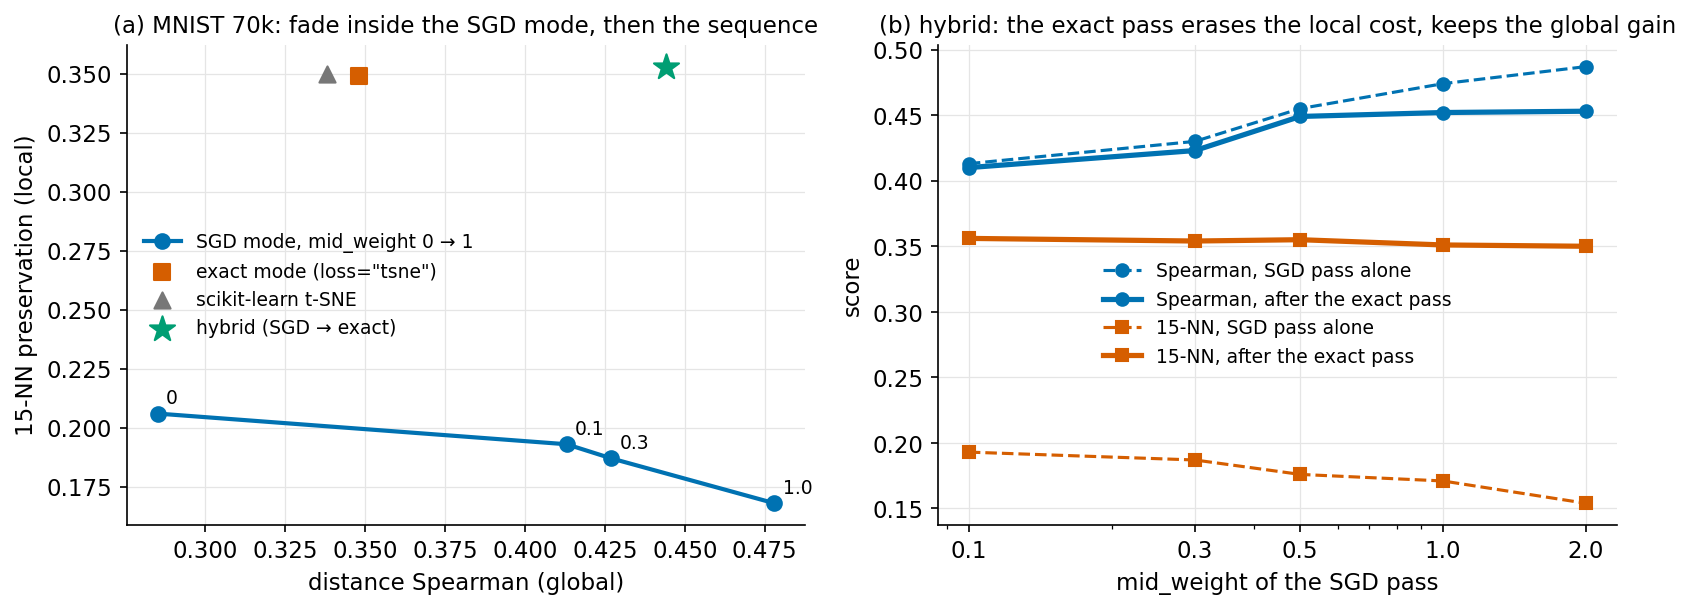
\includegraphics[width=\textwidth]{hybrid.png}
\caption{(a) MNIST 70k, 15-NN against Spearman: the mid-range attraction is the sampled mode's
local/global fade; the full-batch mode sits at the top of the local axis; the hybrid takes the top of
both columns. (b) Scores of the first stage alone (dashed) and after the pass (solid) against the
stiffness $s$ of the first stage.}
\label{fig:hybrid}
\end{figure}

\section{Experiments}\label{sec:exp}
\subsection{Setup}
\emph{Data.} MNIST 70k, Fashion-MNIST 70k, 20 newsgroups ($18.8\mathrm{k} \times 300$ truncated SVD of
the TF-IDF, cosine metric for every method that accepts one, angular for PaCMAP), 15 Gaussian blobs
($10\mathrm{k} \times 200$); graphs: Cora, the US and Europe airport graphs, an SBM with chains, an SBM
with 30k nodes and 782k edges. \emph{Methods}, all at their defaults: UMAP 0.5.12, densMAP, openTSNE
1.0.4, PaCMAP, TriMap, PHATE 2.0, h-NNE, scikit-learn $t$-SNE (Barnes--Hut), $t$-SNE-CUDA 3.0.1 (GPU,
RTX 2070); NCVis could not be built; uwot (R) is not in the panel.

\emph{Metrics.} 15-NN preservation: the exact 15 nearest neighbours in the input space (brute force
over all $n$ points, self excluded) of 5000 query points drawn once per data set, against the exact 15
nearest in the layout over all $n$ points; the mean share retained. Trustworthiness: scikit-learn's at
$k = 15$ on the same 5000 points, both spaces restricted to them; continuity is the same with the two
spaces swapped. Distance Spearman and triplet accuracy: Spearman correlation of the $\binom{2000}{2}$
input and layout distances of a 2000-point sample drawn once per data set, and the share of 200\,000
random triplets of that sample whose distance order is the same in both spaces. Centroid Spearman: the
Spearman correlation of the 45 distances between the class centroids (means of the full 70k) in the two
spaces. 10-NN label accuracy: 5-fold cross-validation of a 10-NN classifier on 10\,000 points of the
layout. Silhouette is reported in the repository as compactness, a look rather than a fidelity, and
omitted here. The evaluation samples are fixed; the only randomness in Table~\ref{tab:seeds} is the
embedding's.

\emph{Timing protocol.} Every method runs with all cores of a 10-core (20-thread) i9-9900X with 54~GB.
The numba methods are warmed up before the clock on data of the same dtype and on 6000 points, enough to
compile the NN-descent path (a float64 warm-up on 500 points leaves two compilations inside the timed
call and had put UMAP at 18~s on MNIST in an earlier version of this table). UMAP and densMAP run
without \texttt{random\_state}: with it their layout is single-threaded (49~s instead of 11~s on MNIST).
PaCMAP's seeded path is also slower (30.6~s against 24.8~s unseeded on MNIST); Table~\ref{tab:seeds}
seeds it and reports the slower time. The main tables (Tables~\ref{tab:mnist}--\ref{tab:blobs}) are means
over 2 seeds (1 on Fashion-MNIST) on a machine shared with other jobs; Table~\ref{tab:seeds} was run
later on an idle machine, with 5 runs per method, and is the reference for every timing and dispersion
statement in the text.

\subsection{Main results}
\begin{table}[t]
\centering\small
\caption{MNIST 70k $\times$ 784, mean over 2 seeds, defaults for every method, best per column in bold;
shared machine.}
\label{tab:mnist}
\resizebox{\textwidth}{!}{\begin{tabular}{lrrrrrr}
\toprule
method & time (s) & 15-NN pres. & trust. & dist. Spearman & triplet acc. & 10-NN acc. \\
\midrule
MAGNET (SGD, default) & \textbf{4.4} & 0.193 & 0.957 & 0.413 & 0.644 & 0.967 \\
MAGNET (\texttt{loss="tsne"}) & 9.2 & 0.349 & 0.966 & 0.348 & 0.627 & 0.966 \\
MAGNET (\texttt{loss="hybrid"}) & 12.5 & \textbf{0.353} & 0.961 & \textbf{0.444} & \textbf{0.656} & 0.960 \\
UMAP 0.5.11 & 18.2 & 0.116 & 0.951 & 0.300 & 0.607 & 0.967 \\
densMAP  & 43.2 & 0.070 & 0.923 & 0.357 & 0.621 & 0.956 \\
openTSNE 1.0.4 & 102.5 & 0.347 & 0.968 & 0.330 & 0.619 & 0.965 \\
PaCMAP & 24.8 & 0.093 & 0.946 & 0.307 & 0.614 & \textbf{0.976} \\
TriMap & 57.0 & 0.088 & 0.933 & 0.184 & 0.597 & 0.964 \\
PHATE 2.0 & 43.2 & 0.080 & 0.865 & 0.291 & 0.611 & 0.861 \\
h-NNE & 9.1 & 0.233 & 0.940 & 0.261 & 0.601 & 0.949 \\
sklearn t-SNE (Barnes-Hut) & 195.7 & 0.350 & \textbf{0.968} & 0.338 & 0.622 & 0.967 \\
t-SNE-CUDA 3.0.1 (GPU) & 13.8 & 0.169 & 0.967 & 0.169 & 0.567 & 0.957 \\
\bottomrule
\end{tabular}
}
\end{table}
\begin{table}[t]
\centering\small
\caption{Fashion-MNIST 70k (1 seed).}\label{tab:fmnist}
\resizebox{\textwidth}{!}{\begin{tabular}{lrrrrrr}
\toprule
method & time (s) & 15-NN pres. & trust. & dist. Spearman & triplet acc. & 10-NN acc. \\
\midrule
MAGNET (SGD, default) & \textbf{4.4} & 0.202 & 0.980 & 0.730 & 0.787 & 0.800 \\
MAGNET (\texttt{loss="tsne"}) & 9.1 & 0.324 & 0.981 & 0.700 & 0.775 & 0.815 \\
MAGNET (\texttt{loss="hybrid"}) & 10.5 & \textbf{0.328} & 0.979 & \textbf{0.752} & \textbf{0.799} & 0.814 \\
UMAP 0.5.12 & 10.9 & 0.133 & 0.975 & 0.571 & 0.728 & 0.778 \\
densMAP  & 38.9 & 0.071 & 0.955 & 0.583 & 0.729 & 0.755 \\
openTSNE 1.0.4 & 98.2 & 0.323 & \textbf{0.983} & 0.617 & 0.732 & 0.817 \\
PaCMAP & 24.2 & 0.099 & 0.971 & 0.581 & 0.729 & 0.773 \\
TriMap & 55.0 & 0.091 & 0.965 & 0.672 & 0.772 & 0.750 \\
PHATE 2.0 & 34.3 & 0.097 & 0.924 & 0.560 & 0.726 & 0.721 \\
h-NNE & 6.6 & 0.173 & 0.912 & 0.490 & 0.698 & 0.805 \\
sklearn t-SNE (Barnes-Hut) & 204.8 & 0.327 & 0.983 & 0.634 & 0.740 & \textbf{0.818} \\
t-SNE-CUDA 3.0.1 (GPU) & 13.9 & 0.235 & 0.975 & 0.269 & 0.614 & 0.811 \\
\bottomrule
\end{tabular}
}
\end{table}
\begin{table}[t]
\centering\small
\caption{20 newsgroups (18.8k $\times$ 300, cosine, 2 seeds).}\label{tab:news20}
\resizebox{\textwidth}{!}{\begin{tabular}{lrrrrrr}
\toprule
method & time (s) & 15-NN pres. & trust. & dist. Spearman & triplet acc. & 10-NN acc. \\
\midrule
MAGNET (SGD, default) & \textbf{1.3} & 0.134 & 0.760 & 0.059 & 0.529 & 0.508 \\
MAGNET (\texttt{loss="tsne"}) & 4.4 & 0.184 & \textbf{0.776} & 0.110 & 0.541 & 0.526 \\
MAGNET (\texttt{loss="hybrid"}) & 4.4 & 0.181 & 0.768 & 0.073 & 0.528 & 0.515 \\
UMAP 0.5.12 & 2.7 & 0.098 & 0.718 & 0.099 & 0.537 & 0.497 \\
densMAP  & 10.7 & 0.068 & 0.658 & 0.123 & 0.545 & 0.443 \\
openTSNE 1.0.4 & 38.8 & 0.187 & 0.772 & 0.106 & 0.542 & \textbf{0.535} \\
PaCMAP & 6.6 & 0.057 & 0.683 & -0.086 & 0.499 & 0.440 \\
TriMap & 12.7 & 0.059 & 0.690 & 0.051 & 0.546 & 0.443 \\
PHATE 2.0 & 20.3 & 0.066 & 0.622 & -0.005 & 0.524 & 0.337 \\
h-NNE & 5.7 & 0.154 & 0.732 & 0.102 & 0.535 & 0.470 \\
sklearn t-SNE (Barnes-Hut) & 48.6 & \textbf{0.192} & 0.742 & \textbf{0.232} & \textbf{0.576} & 0.455 \\
t-SNE-CUDA 3.0.1 (GPU) & 8.5 & 0.148 & 0.651 & 0.039 & 0.517 & 0.333 \\
\bottomrule
\end{tabular}
}
\end{table}
\begin{table}[t]
\centering\small
\caption{15 Gaussian blobs (10k $\times$ 200, 2 seeds).}\label{tab:blobs}
\begin{tabular}{lrrrr}
\toprule
method & time (s) & 15-NN pres. & trust. & dist. Spearman \\
\midrule
MAGNET (SGD, default) & \textbf{1.1} & 0.067 & 0.972 & \textbf{0.690} \\
MAGNET (\texttt{loss="tsne"}) & 2.5 & \textbf{0.126} & 0.974 & 0.505 \\
MAGNET (\texttt{loss="hybrid"}) & 2.5 & 0.124 & 0.974 & 0.684 \\
UMAP 0.5.11 & 2.3 & 0.045 & 0.971 & 0.229 \\
densMAP  & 7.8 & 0.033 & 0.969 & 0.178 \\
openTSNE 1.0.4 & 19.4 & 0.109 & 0.975 & 0.382 \\
PaCMAP & 4.1 & 0.033 & 0.971 & 0.666 \\
TriMap & 7.6 & 0.033 & 0.972 & 0.648 \\
PHATE 2.0 & 24.8 & 0.033 & 0.968 & 0.232 \\
h-NNE & 5.9 & 0.083 & 0.969 & 0.307 \\
sklearn t-SNE (Barnes-Hut) & 17.6 & 0.114 & \textbf{0.975} & 0.381 \\
t-SNE-CUDA 3.0.1 (GPU) & 7.7 & 0.074 & 0.974 & 0.127 \\
\bottomrule
\end{tabular}

\end{table}
\begin{table}[t]
\centering\small
\caption{Five independent runs of the decisive rows on an idle machine (\texttt{seeds.py}; \magnet{},
openTSNE, PaCMAP and scikit-learn seeded 0--4; UMAP unseeded, as seeding it serialises its layout).
Mean $\pm$ standard deviation over the five runs; the dispersion of the mean is that divided by
$\sqrt{5}$. Centroids: Spearman of the 45 inter-centroid distances.}
\label{tab:seeds}
\resizebox{\textwidth}{!}{\begin{tabular}{llrrrrrrrr}
\toprule
data set & method & $n$ & time (s) & 15-NN & trust. & Spearman & triplet & 10-NN acc. & centroids \\
\midrule
MNIST & \magnet{} SGD & 5 & \textbf{4.5 $\pm$ 0.5} & 0.192 $\pm$ 0.002 & 0.956 $\pm$ 0.001 & \underline{0.416 $\pm$ 0.004} & \underline{0.645 $\pm$ 0.001} & 0.966 $\pm$ 0.001 & 0.635 $\pm$ 0.005 \\
MNIST & \magnet{} full-batch & 5 & \underline{6.2 $\pm$ 0.7} & 0.349 $\pm$ 0.001 & \underline{0.966 $\pm$ 0.000} & 0.352 $\pm$ 0.003 & 0.628 $\pm$ 0.001 & 0.966 $\pm$ 0.001 & 0.655 $\pm$ 0.009 \\
MNIST & \magnet{} hybrid & 5 & 8.4 $\pm$ 0.2 & \textbf{0.353 $\pm$ 0.002} & 0.960 $\pm$ 0.001 & \textbf{0.446 $\pm$ 0.014} & \textbf{0.653 $\pm$ 0.004} & 0.961 $\pm$ 0.003 & 0.533 $\pm$ 0.107 \\
MNIST & UMAP 0.5.12 & 5 & 8.4 $\pm$ 0.2 & 0.117 $\pm$ 0.001 & 0.951 $\pm$ 0.001 & 0.299 $\pm$ 0.005 & 0.607 $\pm$ 0.002 & \underline{0.967 $\pm$ 0.001} & \textbf{0.728 $\pm$ 0.014} \\
MNIST & openTSNE 1.0.4 & 5 & 93.5 $\pm$ 0.9 & 0.347 $\pm$ 0.001 & \textbf{0.968 $\pm$ 0.000} & 0.331 $\pm$ 0.002 & 0.620 $\pm$ 0.001 & 0.965 $\pm$ 0.000 & 0.605 $\pm$ 0.001 \\
MNIST & PaCMAP & 5 & 30.5 $\pm$ 0.2 & 0.094 $\pm$ 0.001 & 0.947 $\pm$ 0.001 & 0.310 $\pm$ 0.006 & 0.614 $\pm$ 0.001 & \textbf{0.976 $\pm$ 0.001} & \underline{0.682 $\pm$ 0.008} \\
MNIST & scikit-learn $t$-SNE (BH) & 5 & 186.2 $\pm$ 0.7 & \underline{0.350 $\pm$ 0.000} & \textbf{0.968 $\pm$ 0.000} & 0.338 $\pm$ 0.000 & 0.622 $\pm$ 0.000 & \underline{0.967 $\pm$ 0.000} & 0.663 $\pm$ 0.001 \\
\midrule
Fashion-MNIST & \magnet{} SGD & 5 & \textbf{4.2 $\pm$ 0.3} & 0.204 $\pm$ 0.001 & 0.980 $\pm$ 0.000 & \underline{0.724 $\pm$ 0.002} & \underline{0.784 $\pm$ 0.001} & 0.801 $\pm$ 0.002 & \underline{0.932 $\pm$ 0.007} \\
Fashion-MNIST & \magnet{} full-batch & 5 & \underline{6.4 $\pm$ 0.5} & 0.325 $\pm$ 0.000 & \underline{0.981 $\pm$ 0.000} & 0.698 $\pm$ 0.003 & 0.774 $\pm$ 0.001 & 0.815 $\pm$ 0.001 & 0.890 $\pm$ 0.003 \\
Fashion-MNIST & \magnet{} hybrid & 5 & 8.2 $\pm$ 0.3 & \textbf{0.329 $\pm$ 0.000} & 0.979 $\pm$ 0.000 & \textbf{0.750 $\pm$ 0.003} & \textbf{0.797 $\pm$ 0.001} & 0.813 $\pm$ 0.001 & \textbf{0.934 $\pm$ 0.003} \\
Fashion-MNIST & UMAP 0.5.12 & 5 & 8.1 $\pm$ 0.2 & 0.133 $\pm$ 0.001 & 0.975 $\pm$ 0.001 & 0.579 $\pm$ 0.001 & 0.730 $\pm$ 0.001 & 0.776 $\pm$ 0.003 & 0.883 $\pm$ 0.002 \\
Fashion-MNIST & openTSNE 1.0.4 & 5 & 84.7 $\pm$ 2.2 & 0.323 $\pm$ 0.001 & \textbf{0.983 $\pm$ 0.000} & 0.620 $\pm$ 0.002 & 0.734 $\pm$ 0.001 & \underline{0.816 $\pm$ 0.001} & 0.883 $\pm$ 0.001 \\
Fashion-MNIST & PaCMAP & 5 & 30.2 $\pm$ 0.5 & 0.099 $\pm$ 0.001 & 0.971 $\pm$ 0.000 & 0.582 $\pm$ 0.001 & 0.729 $\pm$ 0.000 & 0.771 $\pm$ 0.002 & 0.883 $\pm$ 0.002 \\
Fashion-MNIST & scikit-learn $t$-SNE (BH) & 5 & 204.3 $\pm$ 31.2 & \underline{0.327 $\pm$ 0.000} & \textbf{0.983 $\pm$ 0.000} & 0.634 $\pm$ 0.000 & 0.740 $\pm$ 0.000 & \textbf{0.818 $\pm$ 0.000} & 0.865 $\pm$ 0.001 \\
\bottomrule
\end{tabular}
}
\end{table}

\paragraph{Sampled mode.} Fastest row on every data set (3.6~s on MNIST over five runs; UMAP 8.4~s,
h-NNE 9.1~s in the shared-machine table), highest pairwise Spearman among neighbour embeddings on
MNIST, Fashion-MNIST and the blobs, 15-NN above UMAP by 60--70\%. h-NNE is the one fast method above
it on 15-NN (0.233 against 0.193) and is behind on every other column.

\paragraph{Full-batch mode.} 15-NN 0.347 $\pm$ 0.001 over five runs against 0.347 $\pm$ 0.001 for
openTSNE and 0.350 for Barnes--Hut $t$-SNE (whose layout is deterministic given its PCA
initialisation: its five runs are identical), in 8.2~s against 93.5 and 186~s. $t$-SNE-CUDA on the GPU takes 13.8~s and is behind on 15-NN and Spearman (0.169
/ 0.169), level on trustworthiness. Trustworthiness is openTSNE's column (0.968 against 0.966).

\paragraph{Hybrid.} Over five runs, 0.353 $\pm$ 0.001 / 0.455 $\pm$ 0.014 on MNIST and 0.328 $\pm$ 0.001
/ 0.750 $\pm$ 0.001 on Fashion-MNIST: the highest 15-NN and the highest pairwise Spearman of the
neighbour embeddings in Table~\ref{tab:seeds} on both data sets. The 15-NN margin over openTSNE
(0.006) is the same as what the pass adds to openTSNE's own layout (0.348 $\to$ 0.354,
Table~\ref{tab:staged}): it is the margin of refining on the 15-NN graph that the metric reads, not of
the sequence. The margin over Barnes--Hut $t$-SNE (0.353 $\pm$ 0.001 against 0.350 on MNIST, 0.328 $\pm$ 0.001
against 0.327 on Fashion-MNIST) is three standard deviations on MNIST and one on Fashion-MNIST. The hybrid's trustworthiness is below openTSNE's
(0.960 against 0.968) and it trails openTSNE at $k = 5$ and $k \ge 50$ (Sec.~\ref{sec:global}). On 20
newsgroups the hybrid's Spearman (0.073) is below UMAP, h-NNE, openTSNE, our full-batch mode (0.110)
and Barnes--Hut (0.232): the sequence does not help on text, and the full-batch mode alone is the better
\magnet{} row there. On the blobs the hybrid is within 0.006 of the best \magnet{} value on each column
without leading either.

\paragraph{Time.} The sequence costs 1.3 times UMAP on MNIST (10.9 against 8.4~s) and 1.2 on
Fashion-MNIST, a ninth of openTSNE and a twentieth of Barnes--Hut. The speed claim is restricted to the
panel and to these data sets.

\paragraph{openTSNE's time.} Its defaults (perplexity 30, hence 90 neighbours, Annoy index, PCA
initialisation, FFT gradient, 250 + 500 iterations at learning rate $n / 12$) were audited phase by
phase in separate runs (\texttt{opentsne\_audit.py}): 24~s of affinities, 2~s of initialisation, 12~s
of early exaggeration, 76~s of main phase (0.15~s per iteration), on the shared machine (the phases
sum to 114~s against 93.5~s end to end on the idle one); \texttt{n\_jobs} 10 or 20 and the
pynndescent index change nothing; 125 + 250 iterations give 15-NN 0.329 in 56~s; uniform $k = 15$
affinities give 0.330 in 100~s. openTSNE is not misconfigured. Where the time differs: its neighbour
search looks for 90 neighbours with Annoy (24~s) where ours looks for 15 with NN-descent (1.2~s), and
its main-phase iteration takes 0.15~s where ours takes 0.015~s at a different layout extent and
schedule (600 iterations against 750). We do not claim a controlled per-component speed-up; the
end-to-end comparison at defaults is the claim.

\subsection{Where the global score comes from}\label{sec:global}
\paragraph{Linear reference.} PCA (truncated SVD on text) to 2-D, scored with the same metrics and
samples (\texttt{baselines\_linear.py}), reaches a distance Spearman of 0.488 on MNIST, 0.873 on
Fashion-MNIST, 0.319 on 20 newsgroups and 0.588 on the blobs, with 15-NN preservation at 0.01--0.03.
Every neighbour embedding is below PCA on the three real sets (hybrid 0.455 / 0.750 / 0.073) and above
it only on the blobs (0.690). ``Highest pairwise Spearman'' in this paper means highest among neighbour
embeddings; the hybrid keeps 93\% of the linear value on MNIST and 86\% on Fashion-MNIST.

\paragraph{Strata and centroids.} Table~\ref{tab:strata} splits the MNIST Spearman by class membership
and by tercile of the input distance, and reduces it to the 45 distances between class centroids. PCA
is ahead on every pairwise stratum; the hybrid ties it on the intermediate tercile (0.132 against
0.131) and is second elsewhere. On the centroids the order reverses: UMAP 0.728 $\pm$ 0.014, PaCMAP
0.682, full-batch 0.658, our sampled mode 0.635 $\pm$ 0.002, openTSNE 0.605, and the hybrid 0.509
$\pm$ 0.075, last of the neighbour embeddings and the one unstable value of Table~\ref{tab:seeds}. The
pass itself moves the centroids by $-0.07$ to $+0.01$ (Table~\ref{tab:staged}); the stiff first stage
starts at 0.52 against 0.635 for the default stiffness. The stiff attraction buys pairwise Spearman at
the expense of the class-level geometry on MNIST; on Fashion-MNIST the hybrid's centroids (0.933 $\pm$
0.002) are level with the sampled mode's and above every other method's. The centroid statistic is
deterministic given a layout; its run-to-run variation here is a property of the stiff first stage.

\paragraph{Neighbourhood scale.} Table~\ref{tab:kscale}: openTSNE leads at $k = 5$ (0.375 against
0.351), the hybrid at $k = 15$ (0.351 against 0.348), openTSNE at $k = 50$ and 100 (0.327 / 0.329 against
0.319 / 0.313). Continuity is 0.944--0.953 for every method, the sampled mode's the highest; the hybrid
has the lowest trustworthiness at $k = 50$ (0.928) and the lowest continuity at $k = 15$ (0.945). The
hybrid's local advantage is at the scale of its graph.

\begin{table}[t]
\centering\small
\caption{Neighbourhood scale on MNIST 70k, same layouts as Fig.~\ref{fig:layouts}: kNN preservation at
$k = 5$ to 100, trustworthiness and continuity at $k = 15$ and 50 (\texttt{extra\_metrics.py}; single
layouts).}
\begin{tabular}{lrrrrrrrr}
\toprule
MNIST 70k & $k=5$ & $k=15$ & $k=50$ & $k=100$ & trust$_{15}$ & cont$_{15}$ & trust$_{50}$ & cont$_{50}$ \\
\midrule
UMAP 0.5.12 & 0.071 & 0.117 & 0.176 & 0.226 & 0.950 & 0.951 & 0.943 & 0.921 \\
openTSNE (FIt-SNE) & \textbf{0.375} & 0.348 & \textbf{0.327} & \textbf{0.329} & \textbf{0.968} & 0.952 & \textbf{0.944} & 0.924 \\
PaCMAP & 0.052 & 0.094 & 0.158 & 0.211 & 0.947 & 0.944 & 0.941 & 0.912 \\
\magnet{} SGD & 0.159 & 0.193 & 0.219 & 0.249 & 0.956 & \textbf{0.953} & 0.941 & \textbf{0.927} \\
\magnet{} full-batch & 0.333 & 0.348 & 0.325 & 0.325 & 0.966 & 0.948 & 0.935 & 0.920 \\
\magnet{} hybrid & 0.351 & \textbf{0.351} & 0.319 & 0.313 & 0.960 & 0.945 & 0.928 & 0.917 \\
\bottomrule
\end{tabular}

\label{tab:kscale}
\end{table}

\begin{table}[t]
\centering\small
\caption{Where the global score comes from, MNIST 70k, same layouts: distance Spearman on the 2000-point
sample split by class membership and by tercile of the input distance (terciles at 9.64 / 10.81), and
Spearman of the 45 inter-centroid distances (\texttt{global\_strata.py}; one layout per method, see
Table~\ref{tab:seeds} for the dispersion of the last column).}
\resizebox{\textwidth}{!}{\begin{tabular}{lrrrrrrr}
\toprule
MNIST 70k, distance Spearman & all & same class & diff.\ class & short & intermediate & long & centroids \\
\midrule
PCA-2 & \textbf{0.488} & \textbf{0.526} & \textbf{0.452} & \textbf{0.392} & 0.131 & \textbf{0.231} & \textbf{0.814} \\
UMAP 0.5.12 & 0.296 & 0.421 & 0.214 & 0.261 & 0.061 & 0.130 & 0.752 \\
openTSNE (FIt-SNE) & 0.329 & 0.483 & 0.250 & 0.320 & 0.073 & 0.090 & 0.607 \\
PaCMAP & 0.306 & 0.412 & 0.228 & 0.287 & 0.068 & 0.108 & 0.684 \\
\magnet{} SGD & 0.418 & 0.466 & 0.362 & 0.364 & 0.108 & 0.127 & 0.635 \\
\magnet{} full-batch & 0.342 & 0.477 & 0.268 & 0.316 & 0.084 & 0.083 & 0.669 \\
\magnet{} hybrid & 0.461 & 0.501 & 0.412 & 0.371 & \textbf{0.132} & 0.158 & 0.421 \\
\bottomrule
\end{tabular}
}
\label{tab:strata}
\end{table}

\subsection{Graphs}
The sampled optimiser takes an adjacency matrix (weights as similarities) with mid-range partners from
short random walks. Table~\ref{tab:graphs} compares it with UMAP's own layout of the same graph
(\texttt{simplicial\_set\_embedding} on the adjacency, spectral initialisation, UMAP's defaults; the
\texttt{metric="precomputed"} route refuses graphs with nodes of degree below \texttt{n\_neighbors}).
Edge preservation of a node is the share of its graph neighbours among its $\deg$ nearest layout
neighbours (exact search, self excluded), averaged over nodes (all nodes below 5000, a fixed sample of
5000 above); 10-NN label accuracy as above. \magnet{} is faster on the four graphs where the times
differ at the displayed precision (a tie on Cora) and keeps more edges on Cora and the airport graphs
(0.51 / 0.35 / 0.33 against 0.47 / 0.23 / 0.27); UMAP keeps more on the SBM with chains (0.535 against
0.483; the adaptive exponent of Appendix~\ref{app:theory} reaches 0.573) and is ahead on the label
accuracy of the airport graphs (0.62 against 0.48 on the US graph), whose labels are activity levels
rather than communities. On the 30k-node SBM both separate the six blocks perfectly and the difference
is the time (1.5~s against 10.4~s on the sparse adjacency). An earlier version of this comparison fed
UMAP the adjacency rows as features, which is not a graph layout and scored 0.26--0.38; it is
withdrawn. Three runs per cell; the standard deviations are at most 0.007 on edge preservation.

\begin{table}[t]
\centering\small
\caption{Graph inputs (\texttt{graph\_table.py}; 3 runs each, all cores; UMAP through
\texttt{simplicial\_set\_embedding} on the adjacency, 500 epochs below 10k nodes and 200 above).}
\label{tab:graphs}
\begin{tabular}{lrrrrrr}
\toprule
graph & \multicolumn{2}{c}{time (s)} & \multicolumn{2}{c}{edge preservation} & \multicolumn{2}{c}{10-NN acc.} \\
 & \magnet{} & UMAP & \magnet{} & UMAP & \magnet{} & UMAP \\
\midrule
Cora (2.7k, 5.3k edges) & \textbf{0.4} & 0.4 & \textbf{0.509} & 0.469 & 0.771 & 0.772 \\
US airports (1.2k, 13.6k) & \textbf{0.1} & 0.9 & \textbf{0.349} & 0.232 & 0.482 & \textbf{0.619} \\
Europe airports (0.4k, 6k) & \textbf{0.1} & 0.7 & \textbf{0.328} & 0.271 & 0.189 & \textbf{0.340} \\
SBM + chains (3k) & \textbf{0.3} & 1.3 & 0.483 & \textbf{0.535} & \textbf{0.849} & 0.810 \\
SBM 30k (782k edges) & \textbf{1.5} & 10.4 & \textbf{0.017} & 0.013 & 1.000 & 1.000 \\
\bottomrule
\end{tabular}

\end{table}

\section{The kernel exponent, in brief}\label{sec:theory}
In the kernel $\phi_b(d) = 1/(1 + a d^{2b})$ the exponent fixes two unrelated things: the near field of
the attraction ($2ab\,d^{2b-1}$ for $d \ll d_k$, while the repulsion is $2b / d$ for every $b$) and the
far field of the repulsion ($2b / (a d^{2b+1})$ for $d \gg d_k$, while the attraction is $2b / d$ for
every $b$). \magnet{} gives them separate values, $b$ (\texttt{kernel\_b}) and $b_r$
(\texttt{repulsion\_b}); at the defaults ($b = 0.6$, $b_r = 1$) and at any half-integer or integer
exponent the \texttt{pow} leaves the inner loop (4.3 against 5.3~s on MNIST; 15-NN 0.192 against 0.189,
within seed noise). Independent attraction and repulsion kernels are the rule in force-directed graph
drawing \citep{fruchterman1991, noack2007energy, jacomy2014forceatlas2}; what is specific to neighbour
embeddings is that one kernel couples the two until it is split.

Appendix~\ref{app:theory} gives two asymptotic arguments and the measurements they are compared with: a
robust-location reading of the near-field attraction under crowding (a direction, sub-quadratic under
crowding and quadratic without, not an optimum; measured optima 0.4--0.5 on crowded data and 1 on
uncrowded synthetic clusters, 0.6--0.7 on text, which it does not explain), and a power-counting reading
of the far-field repulsion (scale-free at $b_r = m/2$ on a homogeneous cloud; on real layouts the
asymptotic window opens only after rescaling, where the per-octave force follows $\alpha - 1 - 2b_r$
with an occupancy exponent $\alpha \approx 1.6$--$1.7$ for MNIST in 2-D and 3-D). A per-point attraction
exponent read off the layout gains 0.01--0.06 of 15-NN on heterogeneous data and nothing on homogeneous
data (Table~\ref{tab:adaptive}).

\section{Related work}
The sequence of Sec.~\ref{sec:staged} is a staged optimisation with an informative start, a family with
several members. \citet{kobak2021init} show that $t$-SNE and UMAP keep the global structure of a PCA or
spectral initialisation; their recipe shrinks the start to $t$-SNE's tiny scale and relies on early
exaggeration, and the global structure it keeps is the linear one. Ours keeps the start at the
full-batch layout's scale and drops the exaggeration, which is what lets a non-linear start's pairwise
Spearman survive (Sec.~\ref{sec:handover}: the tiny scale with exaggeration loses it). PaCMAP
\citep{wang2021pacmap} stages its own optimisation in three phases with mid-near pairs weighted
differently in each; our first stage borrows its mid-near pairs and the annealed weight, and
Sec.~\ref{sec:twobytwo} asks whether PaCMAP's own stages, made stiff, give the same start. Multiscale
affinities \citep{lee2015multiscale} put several scales in one objective rather than in sequence. The
attraction--repulsion spectrum \citep{boehm2022attraction} and the effective loss of negative sampling
\citep{damrich2021umap, damrich2023contrastive} describe what the sampled estimator does to the
objective; our ablation of Sec.~\ref{sec:stagedbase} is consistent with them in that the estimator alone
does not give the first stage its pairwise Spearman. Heavy tails and degrees of freedom
\citep{kobak2020heavy} vary the repulsion's tail with the near field kept quadratic; the split of
Sec.~\ref{sec:theory} varies the two independently. FIt-SNE \citep{linderman2019fitsne} is the
repulsion estimator of our full-batch mode; openTSNE is its reference implementation on the panel.

\section{Limitations}
The result is for two image data sets at 70k points; on text the sequence trails Barnes--Hut $t$-SNE on
pairwise Spearman and the hand-over rule has not been validated at other sizes. The staged baselines of
Table~\ref{tab:staged} are single runs; the seeded $2 \times 2$ design repeats its decisive rows. The
pass drifts: the full-batch objective does not preserve the start's Spearman at convergence
(Sec.~\ref{sec:persist}). PCA keeps the lead on pairwise
Spearman on every real data set, and the stiff attraction that gives the hybrid its pairwise Spearman
makes the class-centroid geometry of MNIST the worst and the most variable of the panel. The hybrid's
local advantage holds at $k = 15$, the scale of its graph, and not at $k = 5$ or $k \ge 50$. The
full-batch and hybrid modes are 2-D only. The lock-free SGD is not bit-reproducible
(\texttt{parallel="owner"} is, at a small cost in 15-NN). The timing comparison is end to end at
defaults; per-component attributions are not controlled, and uwot is absent. The exponent arguments are
asymptotic, give directions rather than optima, and have no window to act in at a layout's working
scale.

\section{Conclusion}
A sampled first stage under a transient mid-range attraction, then a short full-batch $t$-SNE
refinement started at that optimiser's own scale without exaggeration, gives a layout with the
full-batch mode's 15-NN preservation and most of the first stage's pairwise-distance Spearman. The
refinement is generic across the starts we tried and transfers to openTSNE's optimiser; the global
structure it keeps is the start's, and in the first stage that structure is the attraction's, not the
sampled estimator's. The price is paid in class-centroid geometry and in the scales the metric does not
read. The implementation runs the whole sequence in 1.3 times the time of a UMAP layout.

\appendix
\section{Fashion-MNIST layouts}
\begin{figure}[h]
\centering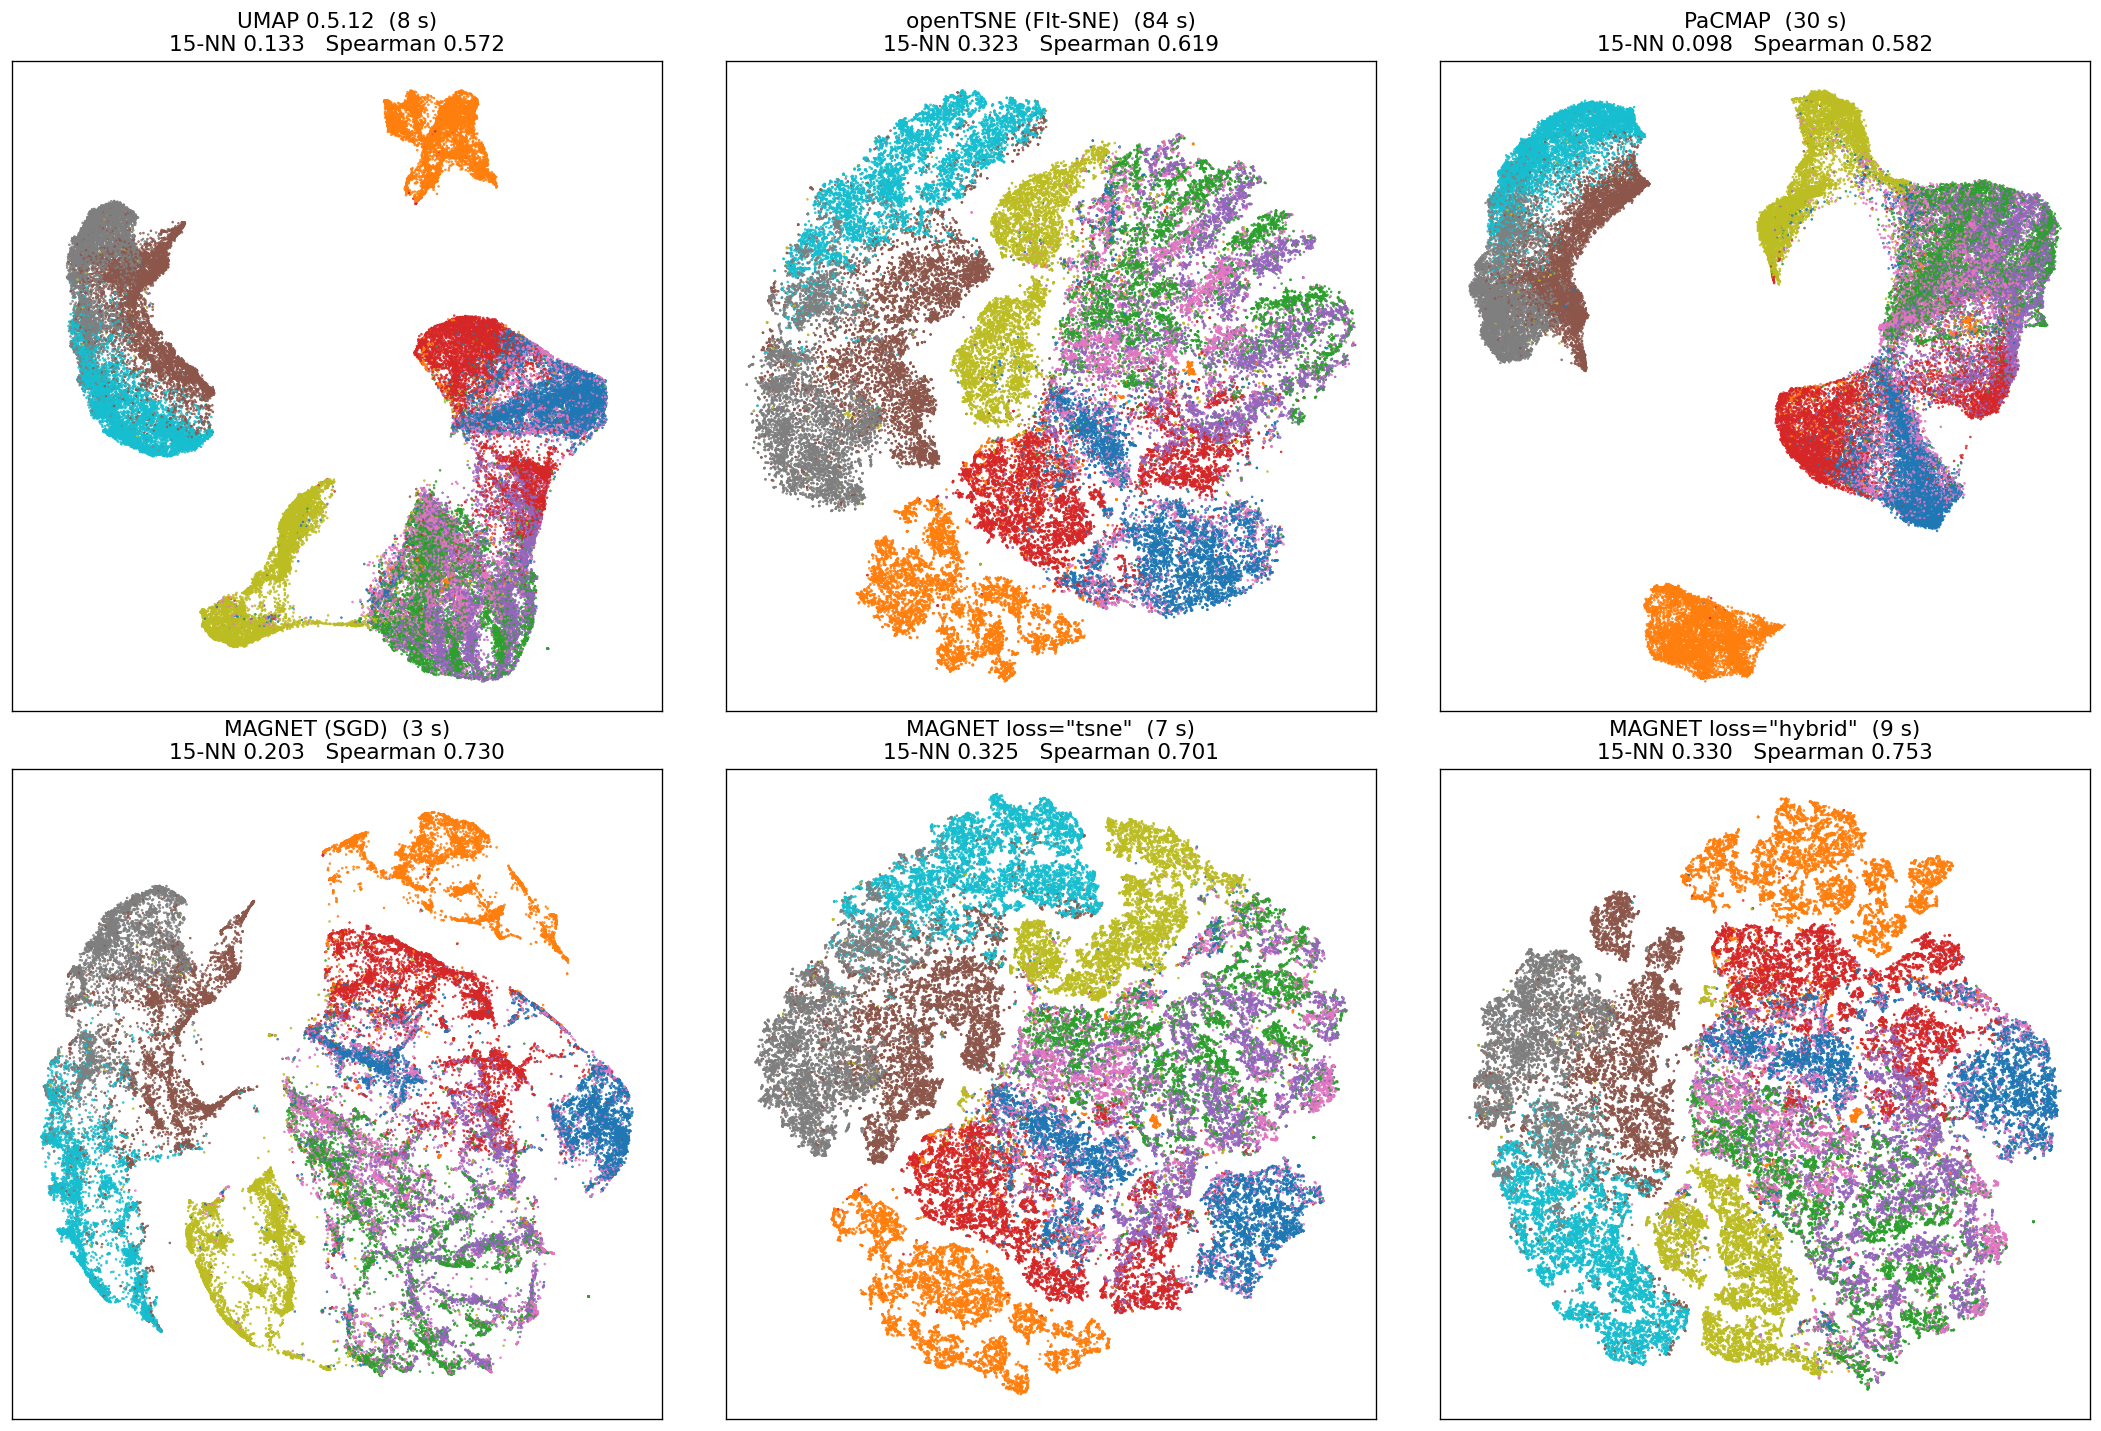
\includegraphics[width=\textwidth]{layouts_fmnist.png}
\caption{Fashion-MNIST 70k under the six methods of Fig.~\ref{fig:layouts}, same protocol (single
runs, idle machine).}
\label{fig:layouts_fmnist}
\end{figure}

\section{Two exponents, two regimes}\label{app:theory}
\subsection{Attraction: a robust location reading}
Under the near-field surrogate $\rho(d) = a d^{2b}$ an edge's equilibrium with a repulsive pull $g$ (the
net far-field repulsion on the point, taken as fixed) sits at $d_{\mathrm{eq}} = (b_r g / ab)^{1/2b}$
with stiffness $4 b b_r g / d_{\mathrm{eq}}^2 > 0$ for every $b$: the exponent does not act through the
stability of a single edge. It acts through crowding. When the intrinsic dimension $q$ exceeds $m$, a
share of the $k$ neighbours cannot sit on the shell and ends in the far field, where every kernel pulls
with $2b / d$. The surrogate is then a location problem in the family $|d|^p$, $p = 2b$: its influence
is bounded in the large-residual tail iff $p \le 1$ and the problem is convex iff $p \ge 1$, and $p = 1$
(the geometric median) is the one exponent with both. Huber's minimax loss says the same: the quadratic
threshold shrinks to zero as the contamination grows. This is an argument on the surrogate, not on the
loss $\log(1 + a d^{2b})$, which is redescending for every $b$ and has a bounded score for every
$b \ge 1/2$, and it says nothing about a jointly moving, repelling configuration: it gives a direction,
sub-quadratic under crowding and quadratic without.

Measured (Fig.~\ref{fig:exponents}a, single runs per point): the best fixed exponent is $1.0 / 0.5 /
0.5 / 0.4 / 0.4$ for synthetic clusters of intrinsic dimension $q = 2 / 3 / 5 / 10 / 20$ in 2-D and
$1.0 / 0.5 / 0.4$ for $q = 3 / 5 / 10$ in 3-D; MNIST and Fashion-MNIST are at 0.5 (contamination 0.24,
the share of kNN edges beyond the kernel scale); the sampled values are consistent with a transition near
$q = m$ but too sparse to establish a step. A Huber kernel has no universal transition scale (best $c$
0.02 on MNIST, 0.2--0.5 on 2-D clusters). Text (20 newsgroups) sits at 0.6--0.7, which the argument does
not explain; hubs and in-degree are ruled out as the cause (Fig.~\ref{fig:exponents}c).

\subsection{Repulsion: which scale carries the loss}
On a homogeneous $m$-dimensional occupancy with $a d^{2b_r} \gg 1$ the far-field loss per octave is
$L[d, 2d] \propto d^{\,m - 2b_r}$: scale-free at $b_r = m/2$, the Cauchy kernel in 2-D, van der Maaten's
$\nu = m - 1$ heuristic recovered. On smooth clouds the per-octave force slopes are $+0.07 / -0.97 /
-2.01 / -3.06$ for $b_r = 0.5 / 1 / 1.5 / 2$ against $0 / -1 / -2 / -3$ (Fig.~\ref{fig:exponents}b). On
real layouts the law needs a window. Binned by the kernel crossover $d_{k,r} = a^{-1/2b_r}$
(Fig.~\ref{fig:tail}), at \magnet{}'s working scale no octave satisfies $a d^{2b_r} > 100$ below half
the layout's radius; binned by the 1-NN distance instead, the fitted octaves sit below the crossover and
the slope is $+0.1$ to $+0.2$ whatever $b_r$ (the mismatch of an earlier version of this analysis).
Rescaled by 16--64 the measured slope follows $\alpha - 1 - 2b_r$ within 0.05, with $\alpha$ the
occupancy exponent of the layout in the window: 1.6--1.7 for MNIST in 2-D and in 3-D, 1.8 / 2.7 for
Gaussian clouds. The measured fidelity optima of $b_r$ are 1.0 in 2-D, 1.0--1.5 in 3-D, 2--4 in 4-D,
3--4 in 6-D: of the order of $m/2$, not fixed by the argument.

\begin{figure}[t]
\centering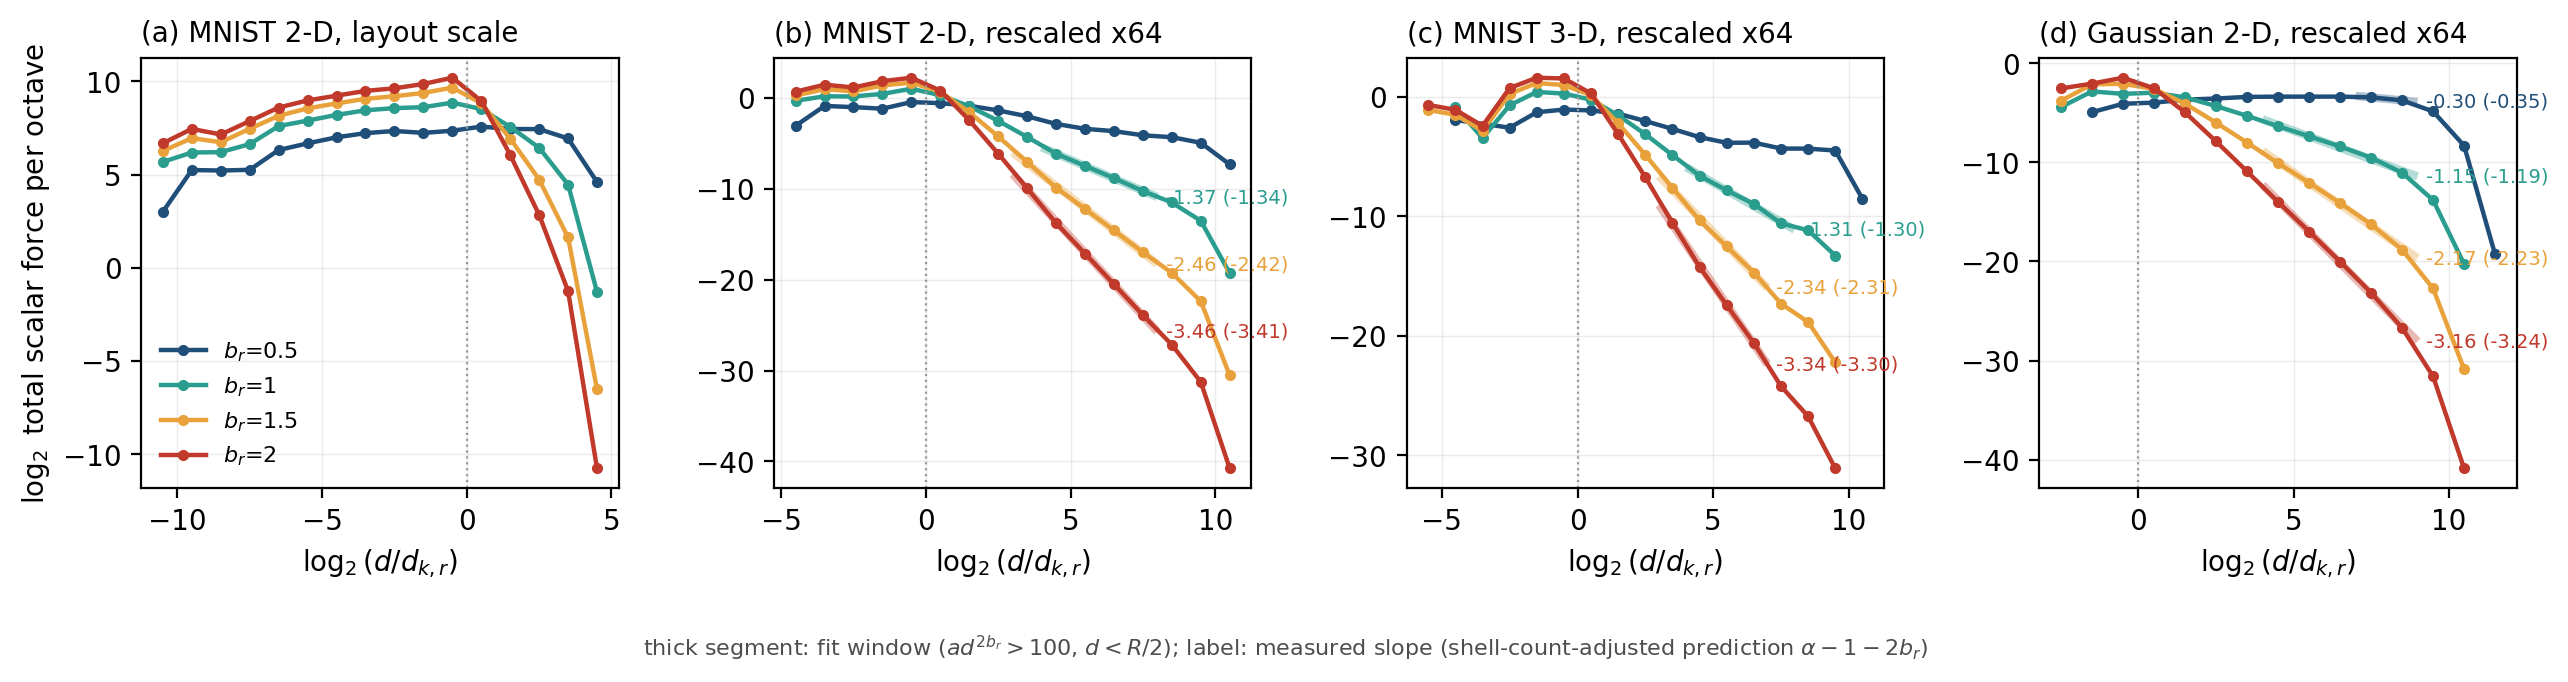
\includegraphics[width=\textwidth]{tail_crossover.png}
\caption{Per-octave repulsive force on fixed layouts against $d / d_{k,r}$ for $b_r = 0.5, 1, 1.5, 2$
(256 anchors against all points). (a) MNIST 20k in 2-D at the layout's own scale: no octave above the
crossover window. (b) The same layout rescaled by 64: slopes $-1.37 / -2.46 / -3.46$ for $b_r = 1 / 1.5
/ 2$ against $\alpha - 1 - 2b_r = -1.34 / -2.42 / -3.41$ with $\alpha = 1.6$. (c) MNIST in 3-D,
$\alpha = 1.7$. (d) Gaussian 2-D cloud, $\alpha = 1.8$.}
\label{fig:tail}
\end{figure}

\begin{figure}[t]
\centering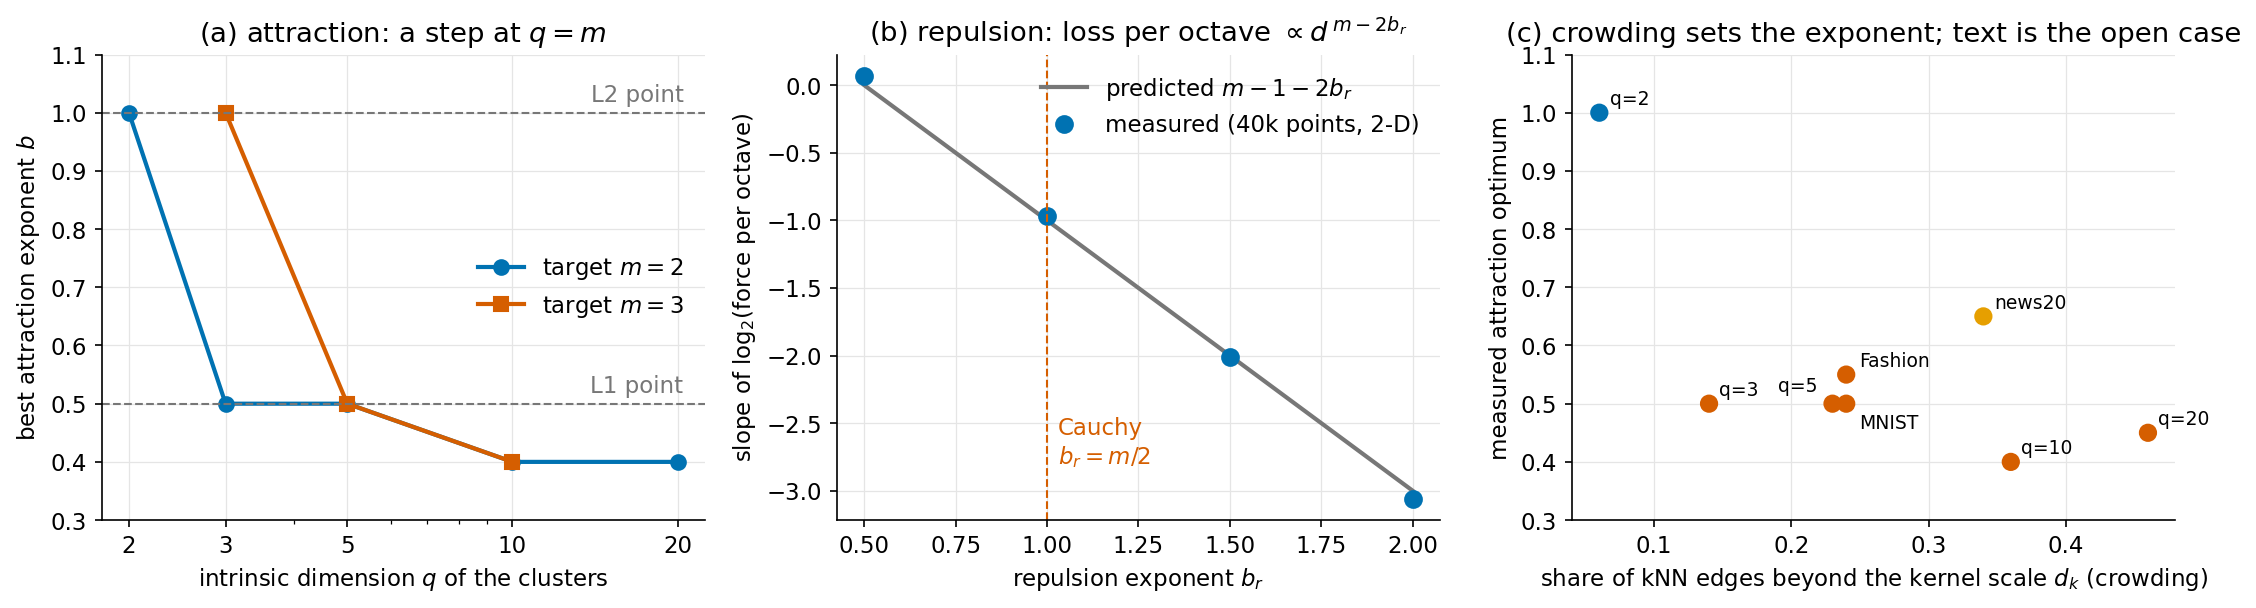
\includegraphics[width=\textwidth]{exponents.png}
\caption{(a) Best attraction exponent against the intrinsic dimension of synthetic clusters. (b)
Per-octave repulsive force on a uniform 2-D cloud: the measured slope follows $m - 1 - 2b_r$. (c)
Measured attraction optimum against the share of kNN edges beyond the kernel scale; image data sit at
$1/2$, text is the open case. Single runs.}
\label{fig:exponents}
\end{figure}

\subsection{Per-point exponent}
An oracle that knows the true $q$ of each point gains 5--10\% of 15-NN over the best fixed exponent on
mixed-dimension data (0.498 $\to$ 0.540, 0.417 $\to$ 0.441 against $b = 0.6$). Two estimators ship:
\texttt{kernel\_b="local"} (a local intrinsic dimension, graph-smoothed, with a step at $m + 0.5$) and
\texttt{kernel\_b="adaptive"} (crowding read off the layout at three quarters of the run as the share of
a point's edges longer than twice the median; the point switches to $L_2$ when none and its degree is
at least 2). Against the fixed exponent $b = 0.6$ that the data would otherwise get, both stay within
0.005 on homogeneous data (MNIST, Fashion-MNIST, 20 newsgroups, Paul15; the US airports graph moves from
0.344 to 0.339) and gain 0.01--0.06 on heterogeneous data (Table~\ref{tab:adaptive}); the best fixed
exponent stays ahead when every point is uncrowded (COIL-20: 0.772 at $b = 1$) and the local-dimension
estimator misses 1-D manifolds.

\begin{table}[t]
\centering\small
\caption{Per-point attraction exponent on heterogeneous data (15-NN kept for data, edge preservation for
graphs; 2--3 runs per cell, means; \texttt{docs/kernel\_exponents.md}, section 4).}
\label{tab:adaptive}
\begin{tabular}{lrrrrrr}
\toprule
data & $b=0.5$ & $b=0.6$ & $b=1$ & oracle & local & adaptive \\
\midrule
1-D + 2-D + 10-D clusters, 6k & 0.493 & 0.498 & 0.474 & 0.540 & \textbf{0.545} & 0.526 \\
5 $\times$ 2-D + 5 $\times$ 10-D, 20k & 0.421 & 0.417 & 0.392 & 0.441 & \textbf{0.459} & 0.442 \\
COIL-20 & 0.694 & 0.717 & \textbf{0.772} & & 0.701 & 0.720 \\
MNIST 20k & 0.292 & 0.282 & 0.200 & & 0.294 & 0.291 \\
Cora graph & 0.442 & 0.507 & 0.470 & & & \textbf{0.522} \\
US airports graph & 0.333 & 0.344 & 0.297 & & & 0.339 \\
SBM + chains & 0.449 & 0.484 & 0.532 & 0.571 & & \textbf{0.573} \\
\bottomrule
\end{tabular}
\end{table}

\section{Implementation}\label{app:impl}
\paragraph{Where the SGD time goes.} On MNIST 70k the default fit is 1.1~s of kNN graph, 0.9~s of graph
construction and spectral initialisation, and 2--3~s of SGD. One thread runs the SGD at 39 core-cycles
per force evaluation, but 10 cores give only $3.7\times$: with lock-free updates every sampled edge
writes cache lines owned by other cores and the slowest thread paces each epoch. The alternative
\texttt{parallel="owner"} mode gives each thread a chunk of nodes to write and a per-epoch snapshot to
read: it halves the SGD time (1.45 against 2.98~s), is bit-reproducible for any thread count, and shifts
the balance towards pairwise Spearman (0.451 against 0.415, 15-NN 0.189 against 0.193). It is not the
default because the hybrid's attraction is tuned for the lock-free mode.

\paragraph{Sparse inputs.} The sparse NN-descent scatters the row about to be compared against many
partners into a dense per-thread buffer once; every partner's dot product is then a branch-free gather
over its own non-zeros. The kNN graph of 20 newsgroups TF-IDF ($18.8\mathrm{k} \times 24\mathrm{k}$, 57
non-zeros per row) takes 0.67~s instead of 2.3~s at the same recall (0.86 of the exact 15-NN), the fit
1.6~s (UMAP 4.5~s). This is a different representation from the SVD-300 of the main tables and is a
timing, not a fidelity, comparison. Dense projections of the rows followed by a dense search keep
12--37\% of the true neighbours.

\paragraph{Cost.} 1M points (50 anisotropic clusters in 50-D) in 44~s and 3.3~GB on 20 threads
(Fig.~\ref{fig:scaling}); the full-batch mode takes 17~s at 250k and 56~s at 1M. \texttt{transform()}
places 10k MNIST test points in 0.6~s at 0.96 of 10-NN accuracy (UMAP 14.8~s).

\begin{figure}[t]
\centering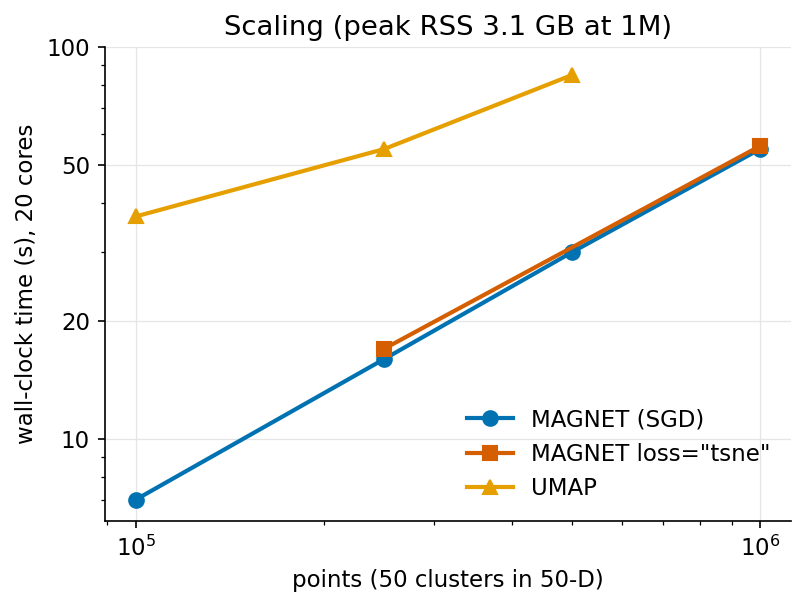
\includegraphics[width=0.5\textwidth]{scaling.png}
\caption{Wall-clock time against the number of points (50 anisotropic clusters in 50-D, 20 threads).}
\label{fig:scaling}
\end{figure}

\paragraph{FFT repulsion accuracy.} Against the exact all-pairs sum in double precision on the hybrid's
own MNIST layout (\texttt{k16\_fft\_check.py}; subsamples of 5k and 20k points, and the full 70k), the
default grid (3 interpolation points per box of width 1, 163 boxes a side at this extent) gives $Z$ to
0.06--0.3\%, the per-point repulsive force to 2.8--4\% RMS (relative to the RMS force; worst point
21--32\%), and a cosine of 0.9992--0.9996 between the interpolated and the exact force fields. Five
interpolation points per box give 0.2--0.4\% RMS and a cosine above 0.99999 at 1.7 times the cost; box
width 1.5 (the speed preset) gives 10--14\% RMS. These are the accuracies of the
FIt-SNE scheme at its usual settings; the pass is accurate to its grid, not exact, which is why the
paper says full-batch.

\bibliographystyle{plainnat}
\begin{thebibliography}{99}\small
\bibitem[B\"ohm et al.(2022)]{boehm2022attraction} J. N. B\"ohm, P. Berens, D. Kobak. Attraction-repulsion spectrum in neighbor embeddings. JMLR 23, 2022.
\bibitem[Damrich and Hamprecht(2021)]{damrich2021umap} S. Damrich, F. A. Hamprecht. On UMAP's true loss function. NeurIPS 2021.
\bibitem[Damrich et al.(2023)]{damrich2023contrastive} S. Damrich, J. N. B\"ohm, F. A. Hamprecht, D. Kobak. From $t$-SNE to UMAP with contrastive learning. ICLR 2023.
\bibitem[Kobak et al.(2020)]{kobak2020heavy} D. Kobak, G. Linderman, S. Steinerberger, Y. Kluger, P. Berens. Heavy-tailed kernels reveal a finer cluster structure in $t$-SNE visualisations. ECML-PKDD 2019.
\bibitem[Linderman et al.(2019)]{linderman2019fitsne} G. C. Linderman, M. Rachh, J. G. Hoskins, S. Steinerberger, Y. Kluger. Fast interpolation-based $t$-SNE for improved visualization of single-cell RNA-seq data. Nature Methods 16, 2019.
\bibitem[McInnes et al.(2018)]{mcinnes2018umap} L. McInnes, J. Healy, J. Melville. UMAP: uniform manifold approximation and projection for dimension reduction. arXiv:1802.03426.
\bibitem[Fruchterman and Reingold(1991)]{fruchterman1991} T. M. J. Fruchterman, E. M. Reingold. Graph drawing by force-directed placement. Software: Practice and Experience 21(11), 1991.
\bibitem[Jacomy et al.(2014)]{jacomy2014forceatlas2} M. Jacomy, T. Venturini, S. Heymann, M. Bastian. ForceAtlas2, a continuous graph layout algorithm for handy network visualization designed for the Gephi software. PLoS ONE 9(6), 2014.
\bibitem[Kobak and Linderman(2021)]{kobak2021init} D. Kobak, G. C. Linderman. Initialization is critical for preserving global data structure in both $t$-SNE and UMAP. Nature Biotechnology 39, 2021.
\bibitem[Lee et al.(2015)]{lee2015multiscale} J. A. Lee, D. H. Peluffo-Ord\'o\~nez, M. Verleysen. Multi-scale similarities in stochastic neighbour embedding: reducing dimensionality while preserving both local and global structure. Neurocomputing 169, 2015.
\bibitem[Noack(2007)]{noack2007energy} A. Noack. Energy models for graph clustering. Journal of Graph Algorithms and Applications 11(2), 2007.
\bibitem[van der Maaten and Hinton(2008)]{vandermaaten2008tsne} L. van der Maaten, G. Hinton. Visualizing data using $t$-SNE. JMLR 9, 2008.
\bibitem[Wang et al.(2021)]{wang2021pacmap} Y. Wang, H. Huang, C. Rudin, Y. Shaposhnik. Understanding how dimension reduction tools work: an empirical approach to deciphering $t$-SNE, UMAP, TriMap, and PaCMAP for data visualization. JMLR 22, 2021.
\end{thebibliography}
\end{document}
